\documentclass{beamer}
\usepackage{graphicx}
\usepackage{tikz}
\usetikzlibrary{shapes,arrows}
\usepackage{tikz}
%\usecolortheme{seahorse}
  \setbeamertemplate{footline}[page number]
\usepackage{multirow}
\setbeamertemplate{navigation symbols}{}
\setbeamertemplate{frametitle}[default][center]
\setbeamerfont{frametitle}{shape=\scshape}
\usepackage{color}

\usepackage{csquotes}

\usepackage{xcolor}

\usepackage[flushleft]{threeparttable}

{\title{\textsc{Econ 352 - Economic Growth: Malthus and Solow} \\ \tiny (See Williamson Ch. 7)}
\author{Trevor S. Gallen}
\date{}
\begin{document}
\renewcommand*{\inserttotalframenumber}{\pageref{lastframe}}


\setbeamertemplate{caption}{\raggedright\insertcaption\par}

\begin{frame}
\titlepage
\end{frame}

\begin{frame}
\frametitle[alignment=center]{Introduction}
\begin{itemize}
\item We've seen some one-period models of Macro
\bigskip
\item But we want to understand growth  
\bigskip
\item Let's start with growth facts and move on to a theory
\end{itemize}
\end{frame}

\begin{frame}
\frametitle[alignment=center]{Growth Facts}
\begin{enumerate}
\item Before the Industrial Revolution (roughly 1800), living standards across time and countries did not vary much (everyone was poor)
\bigskip
\item Since then, per-capita income growth has bee sustained in the richest countries (roughly 2\%/year in the US since 1900)
\bigskip
\item There's a positive correlation between investment and output per worker
\bigskip
\item There's a negative correlation between population growth and output per worker
\end{enumerate}
\end{frame}

\begin{frame}
\frametitle[alignment=center]{Growth Facts}
\begin{enumerate}\addtocounter{enumi}{4}
\item Differences in per-capita income exploded between 1800 and 1950
\bigskip
\item There is no correlation between level of output in 1960 and growth in per capita for the years 1960-2019
\bigskip
\item Richer countries are much more alike in terms of rates of growth of real per capita income than are poor countries
\end{enumerate}
Let's see!
\end{frame}

\begin{frame}
\frametitle[alignment=center]{Growth Took Off!}
\begin{figure}
\centering
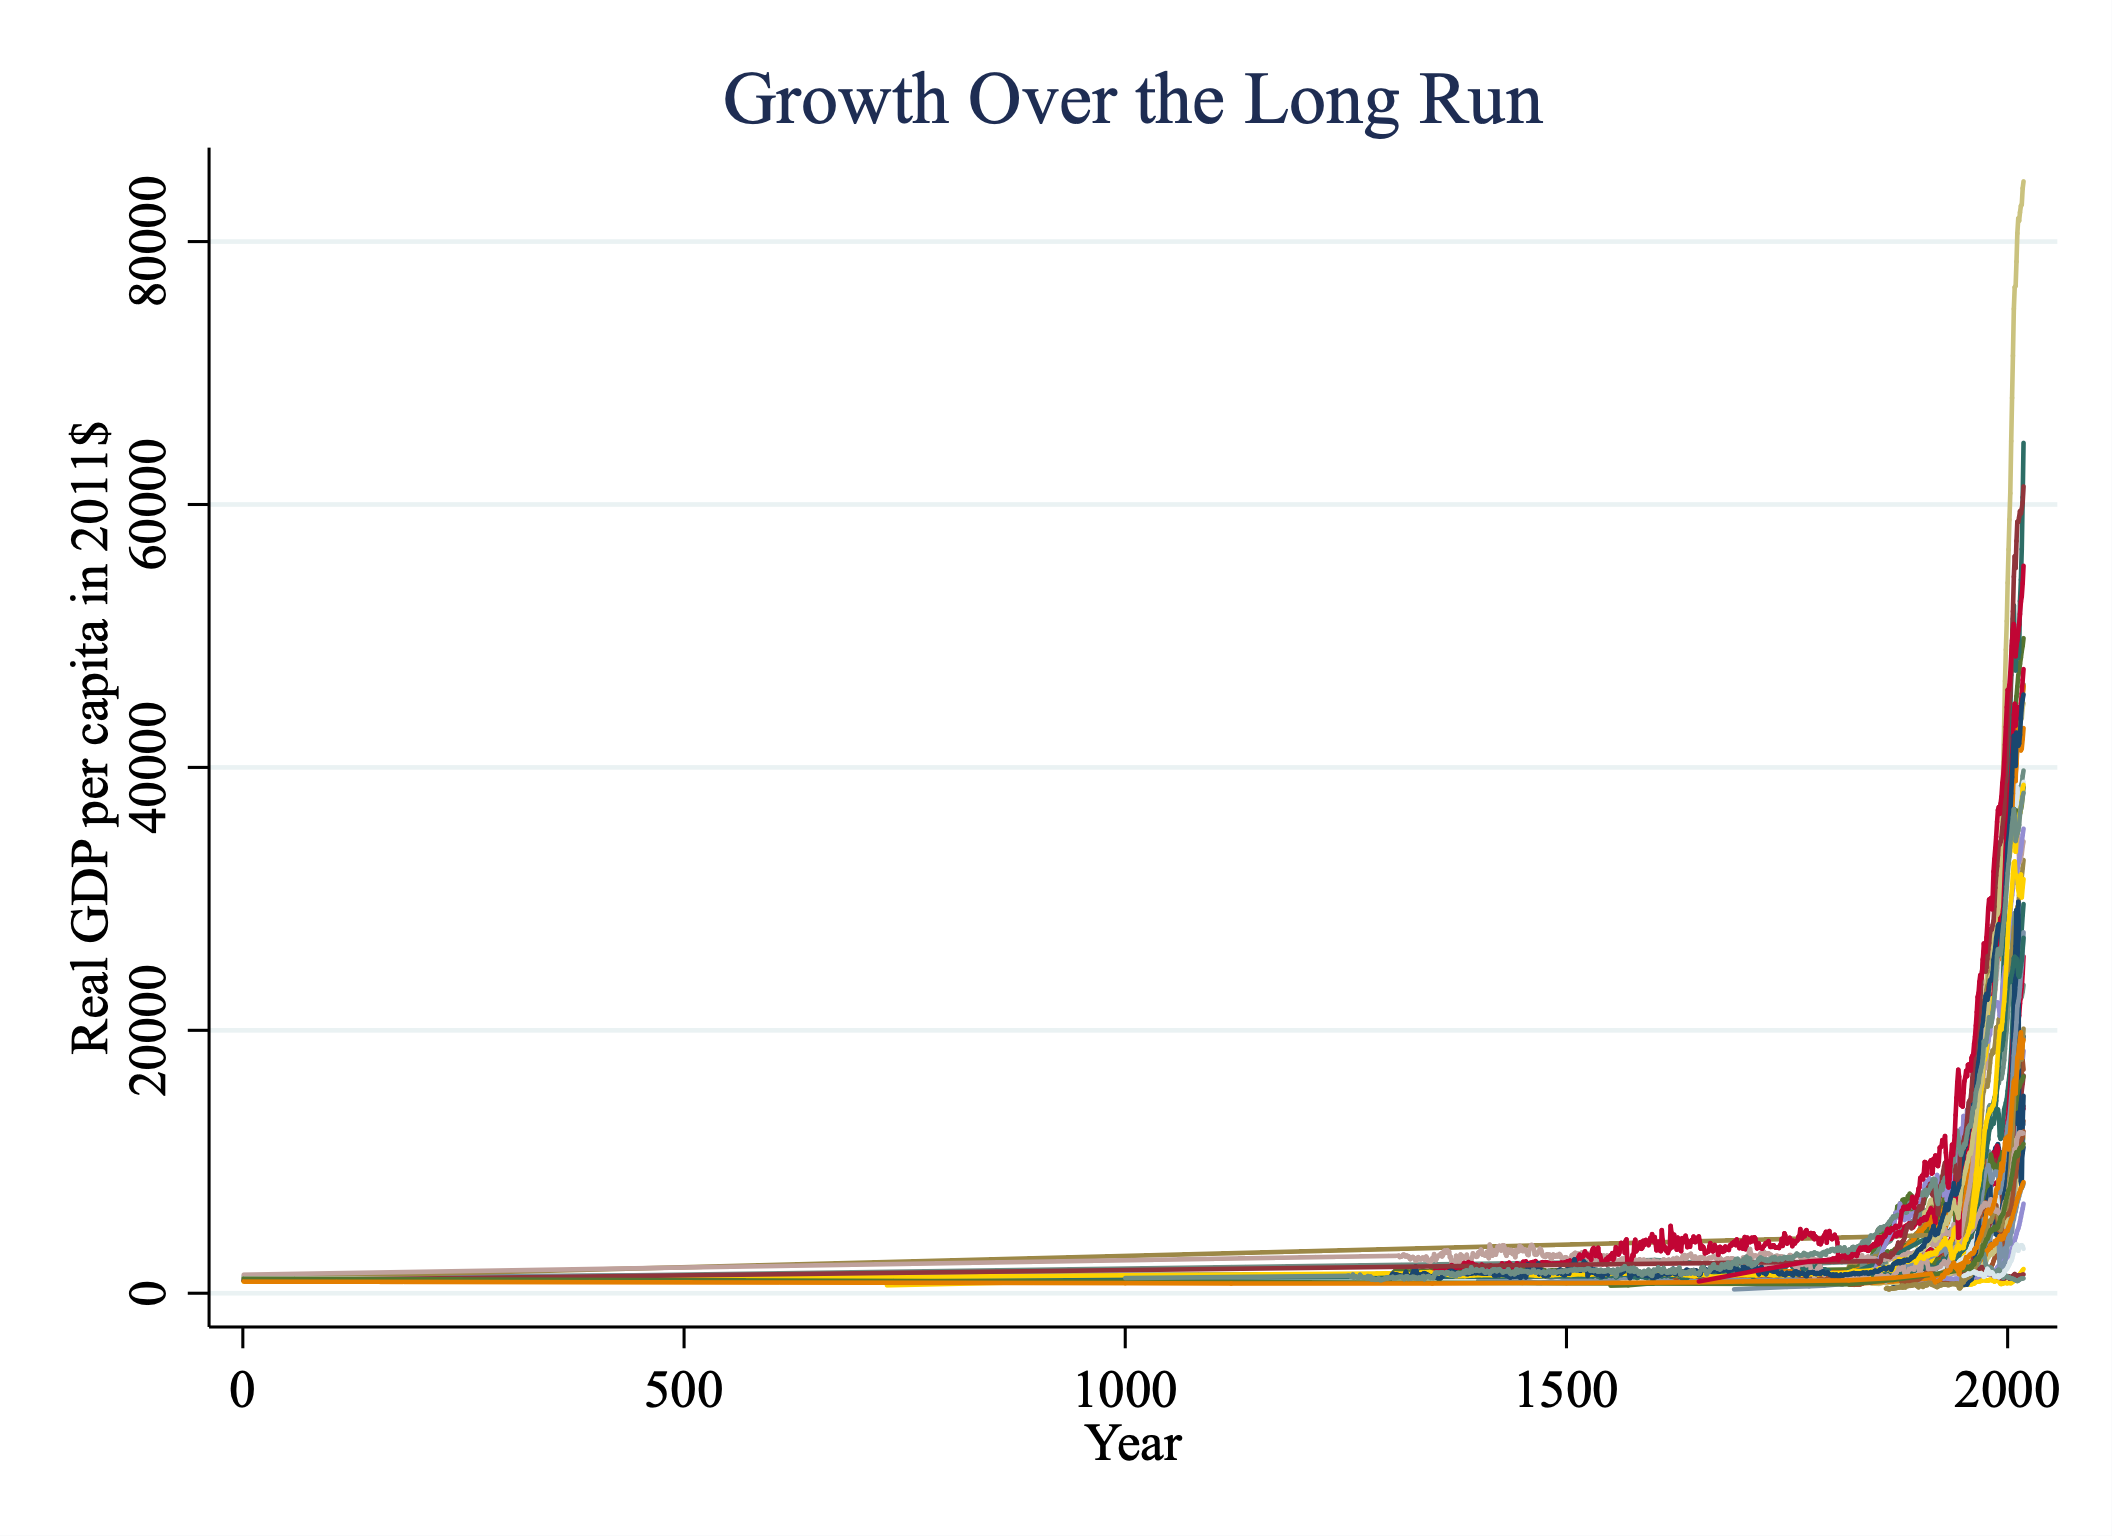
\includegraphics[scale=0.2]{Figures/Fig_7pt0a.png}
\end{figure}
Growth is positively correlated with investment
\end{frame}

\begin{frame}
\frametitle[alignment=center]{As did disparities between countries}
\begin{figure}
\centering
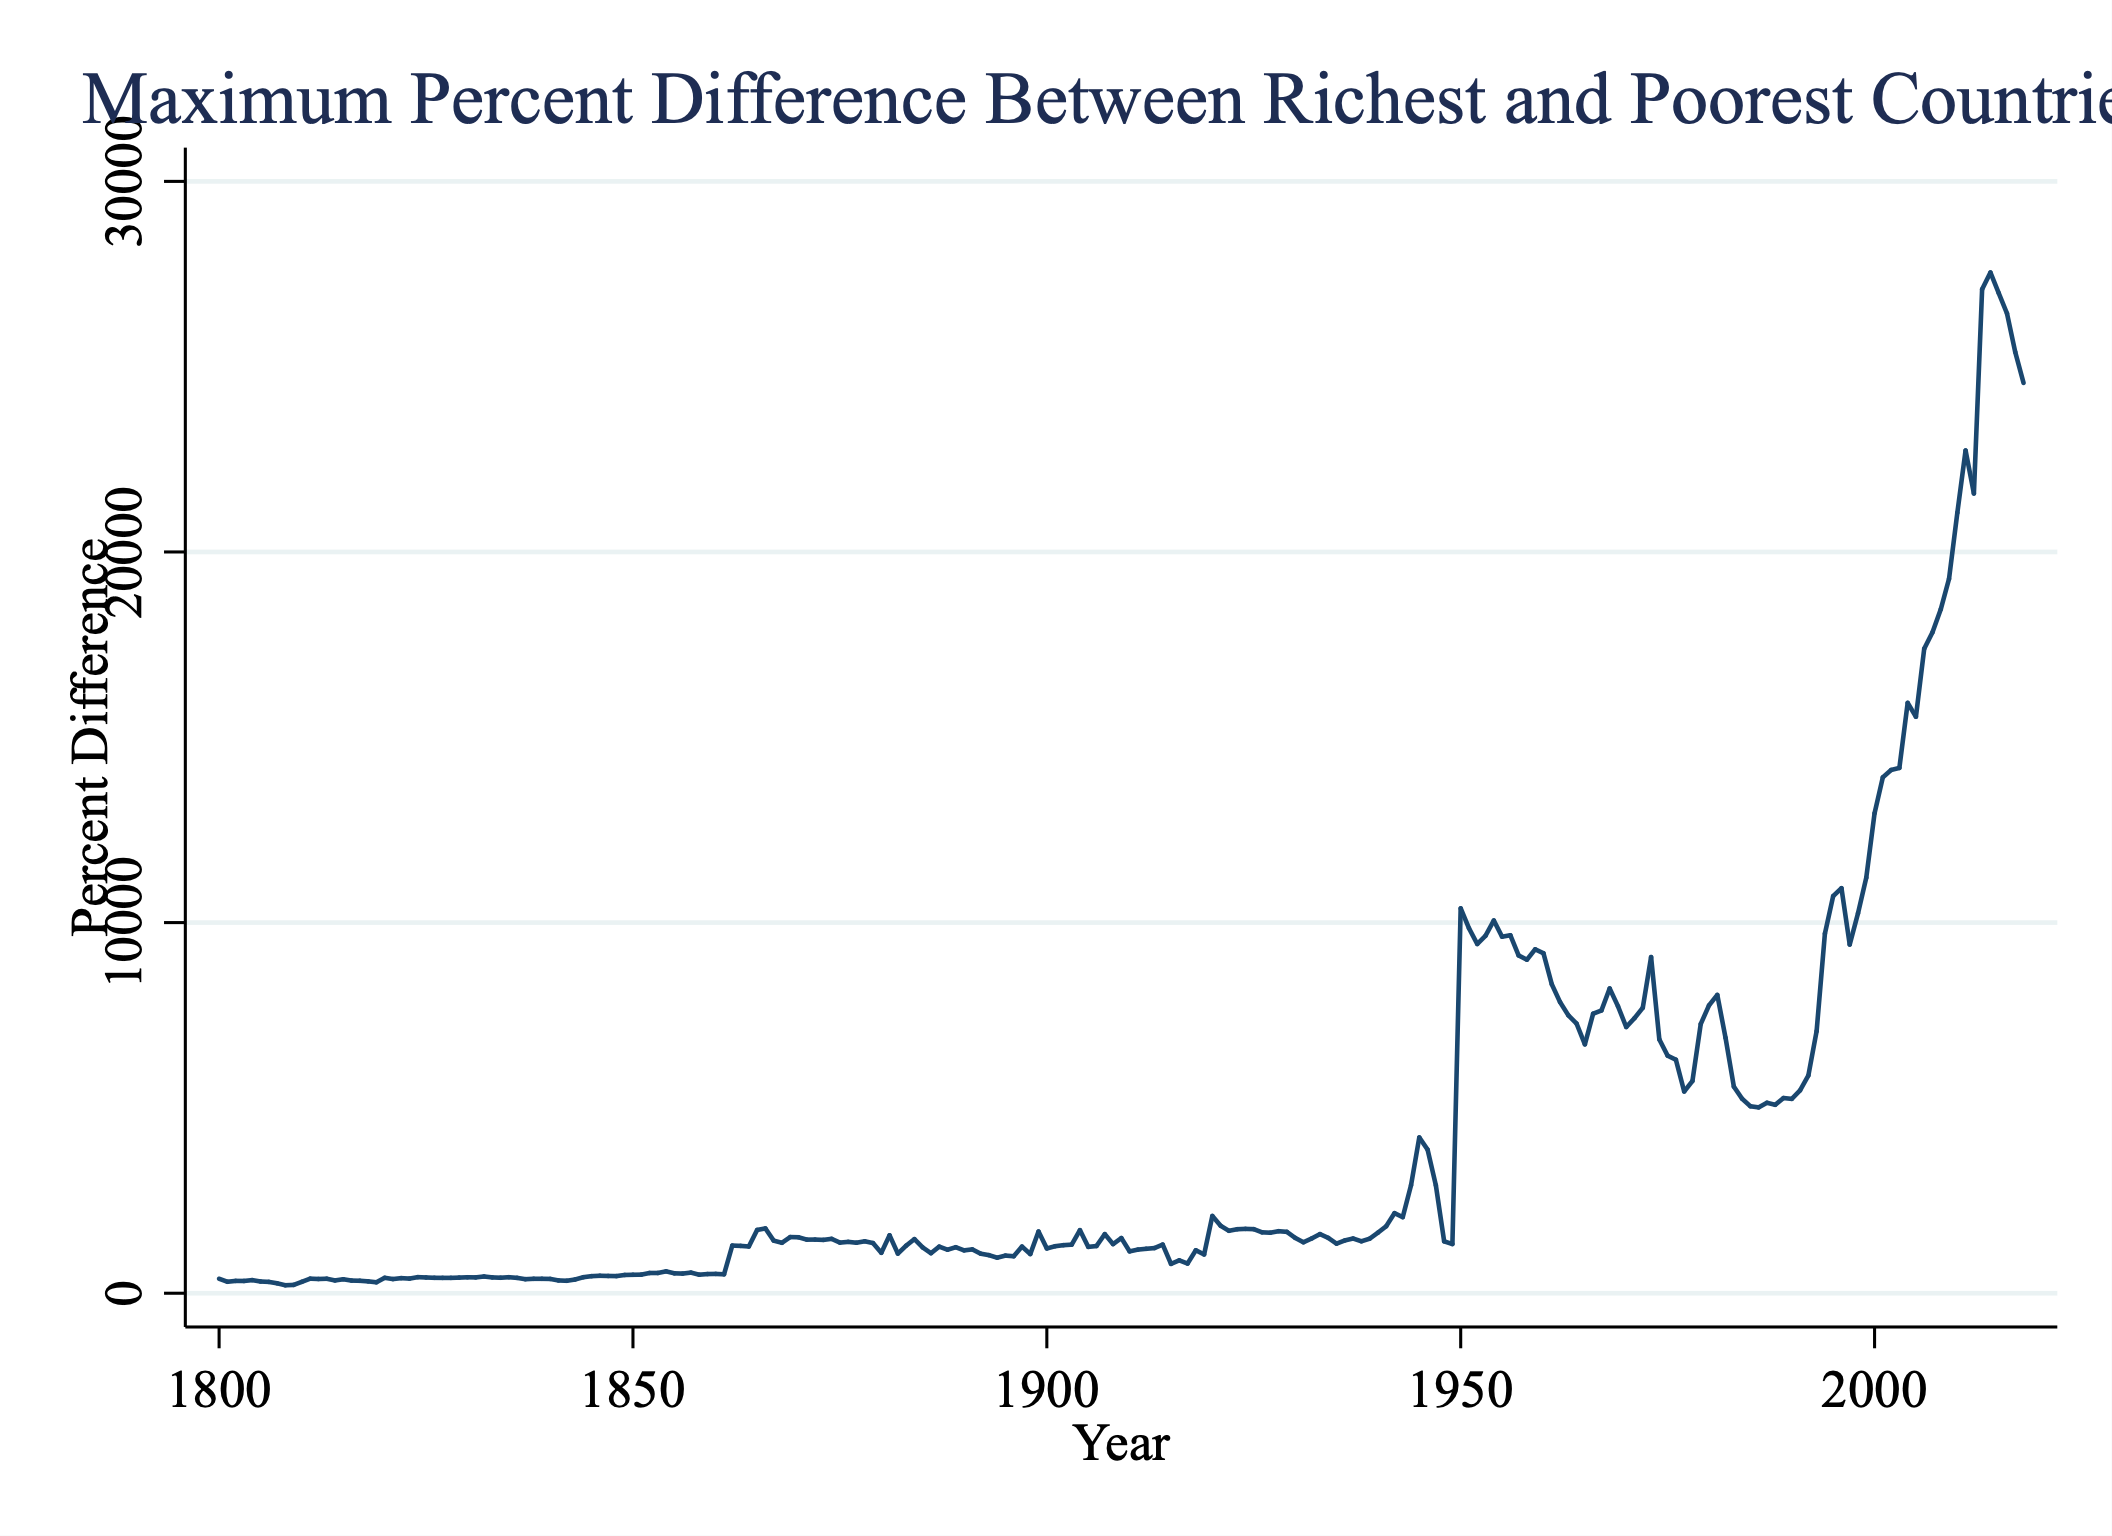
\includegraphics[scale=0.25]{Figures/Fig_7pt0b.png}
\end{figure}
Growth is positively correlated with investment
\end{frame}

\begin{frame}
\frametitle[alignment=center]{Though almost all countries have grown}
\begin{figure}
\centering
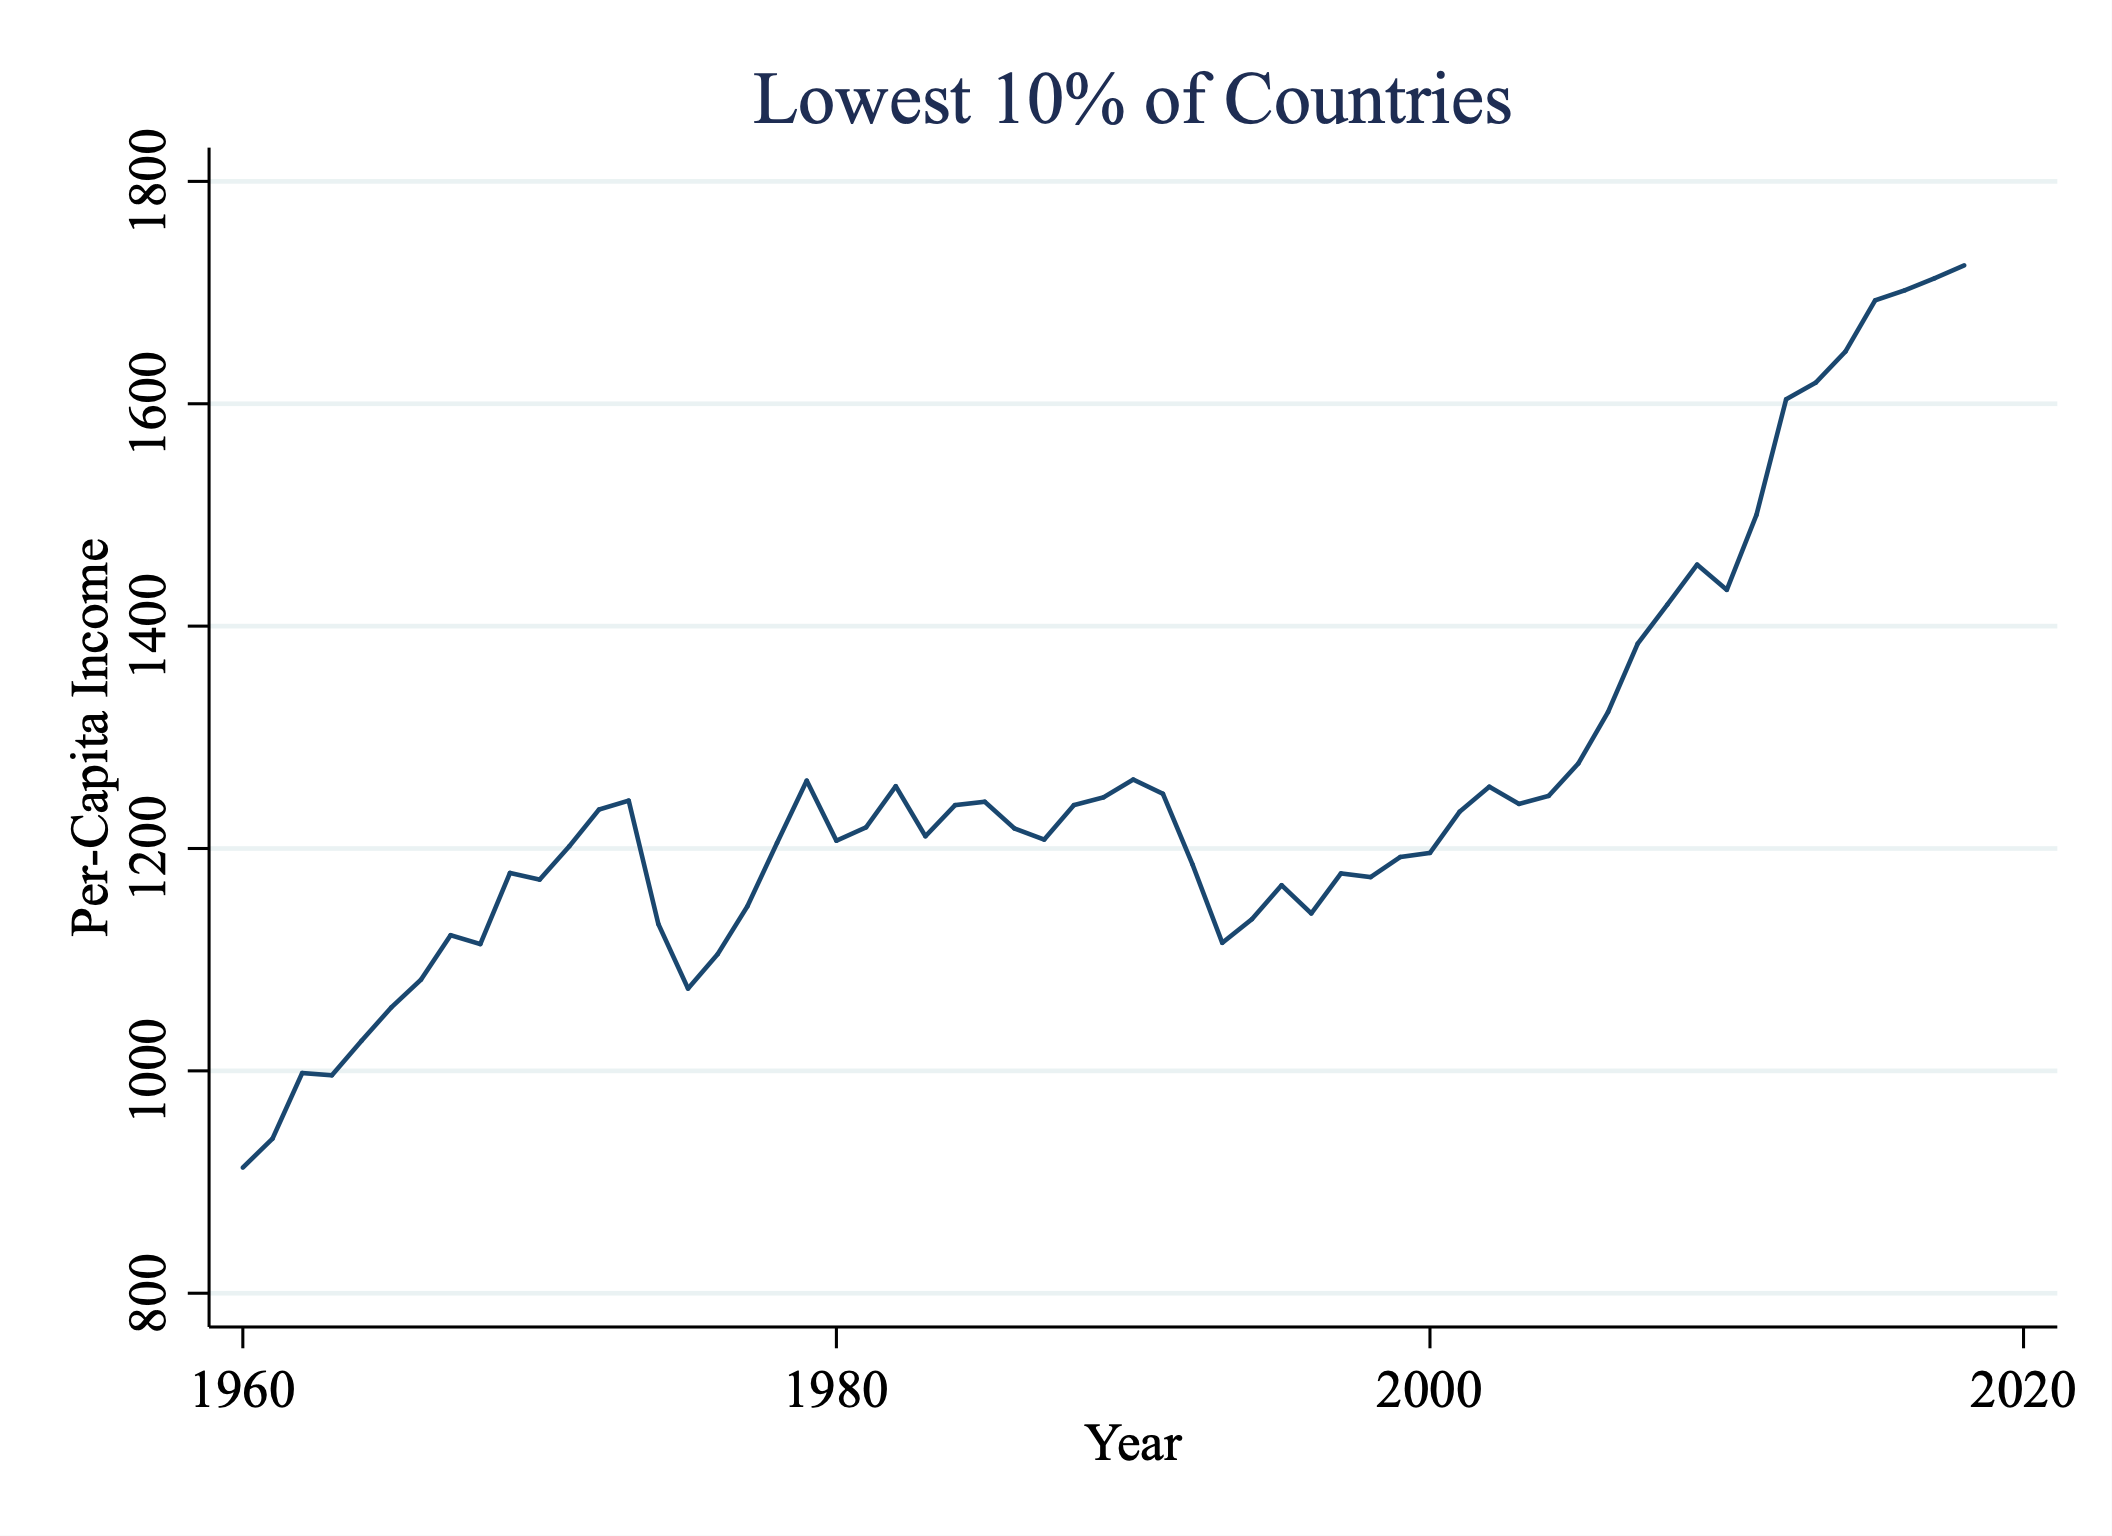
\includegraphics[scale=0.25]{Figures/Fig_7pt0c.png}
\end{figure}
Growth is positively correlated with investment
\end{frame}


\begin{frame}
\frametitle[alignment=center]{Growth is positively correlated with investment}
\begin{figure}
\centering
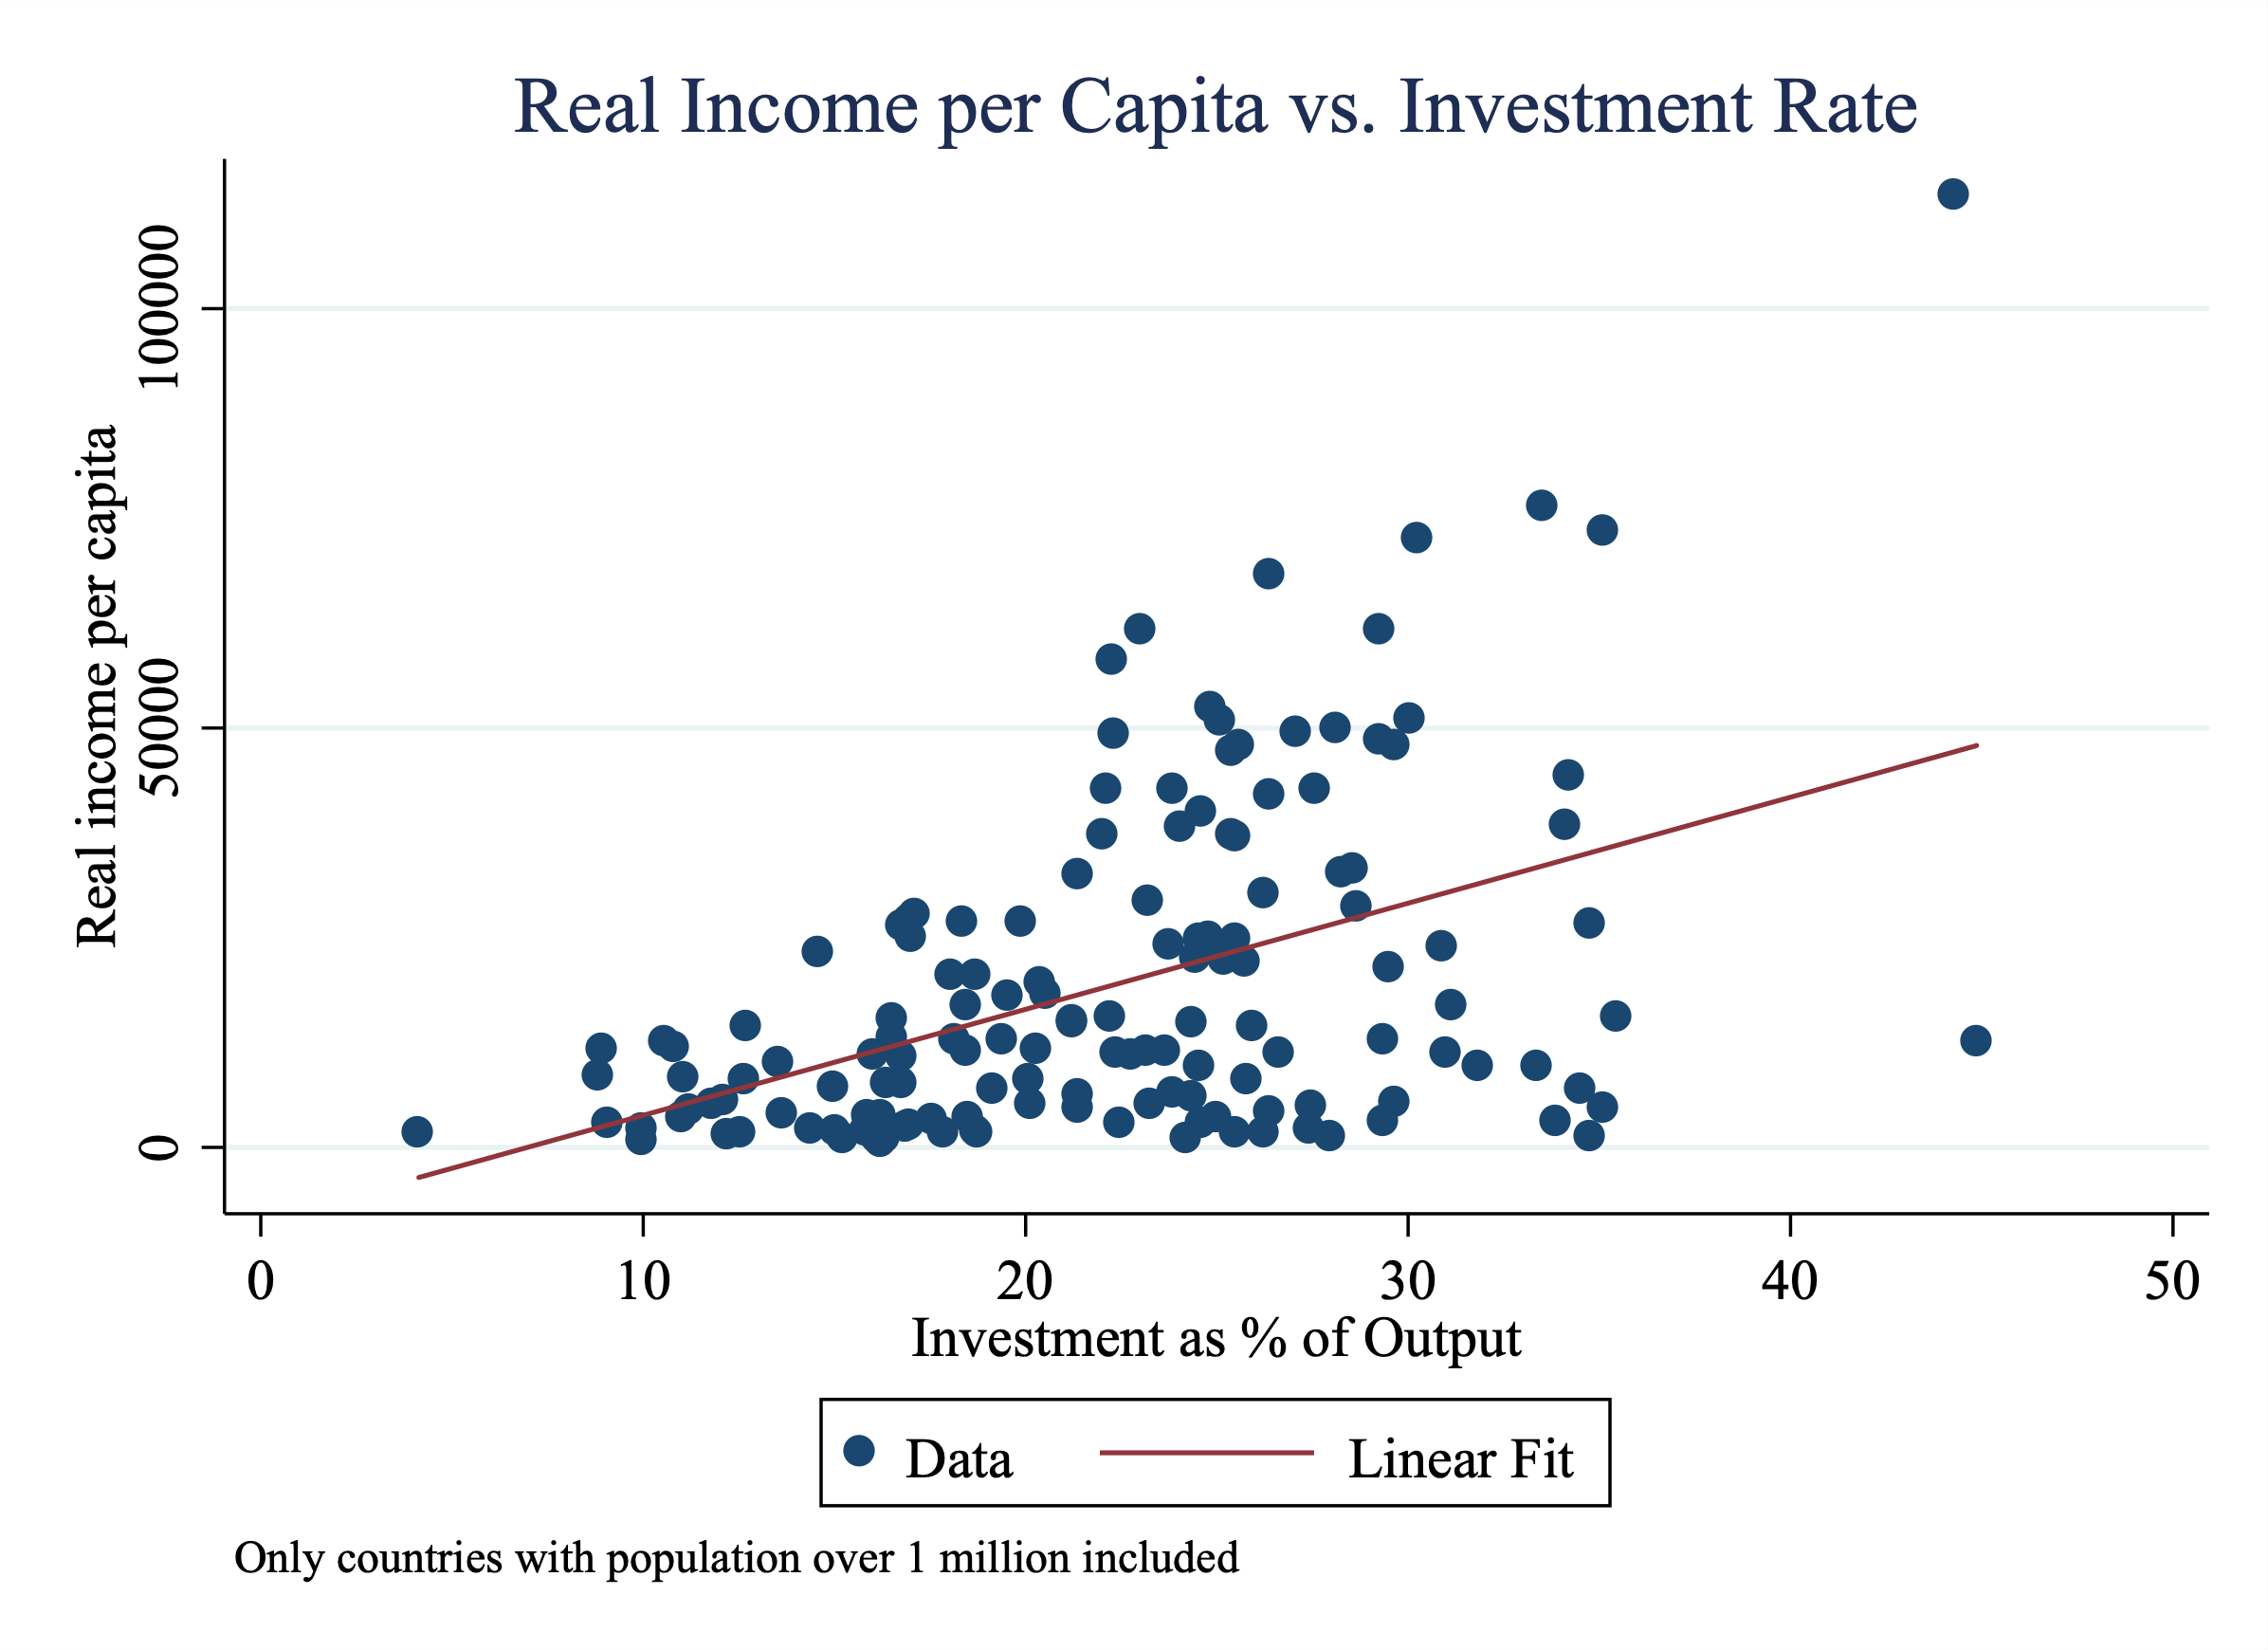
\includegraphics[scale=0.25]{Figures/Fig_7pt1.png}
\end{figure}

\end{frame}

\begin{frame}
\frametitle[alignment=center]{Growth is negatively correlated with population growth}
\begin{figure}
\centering
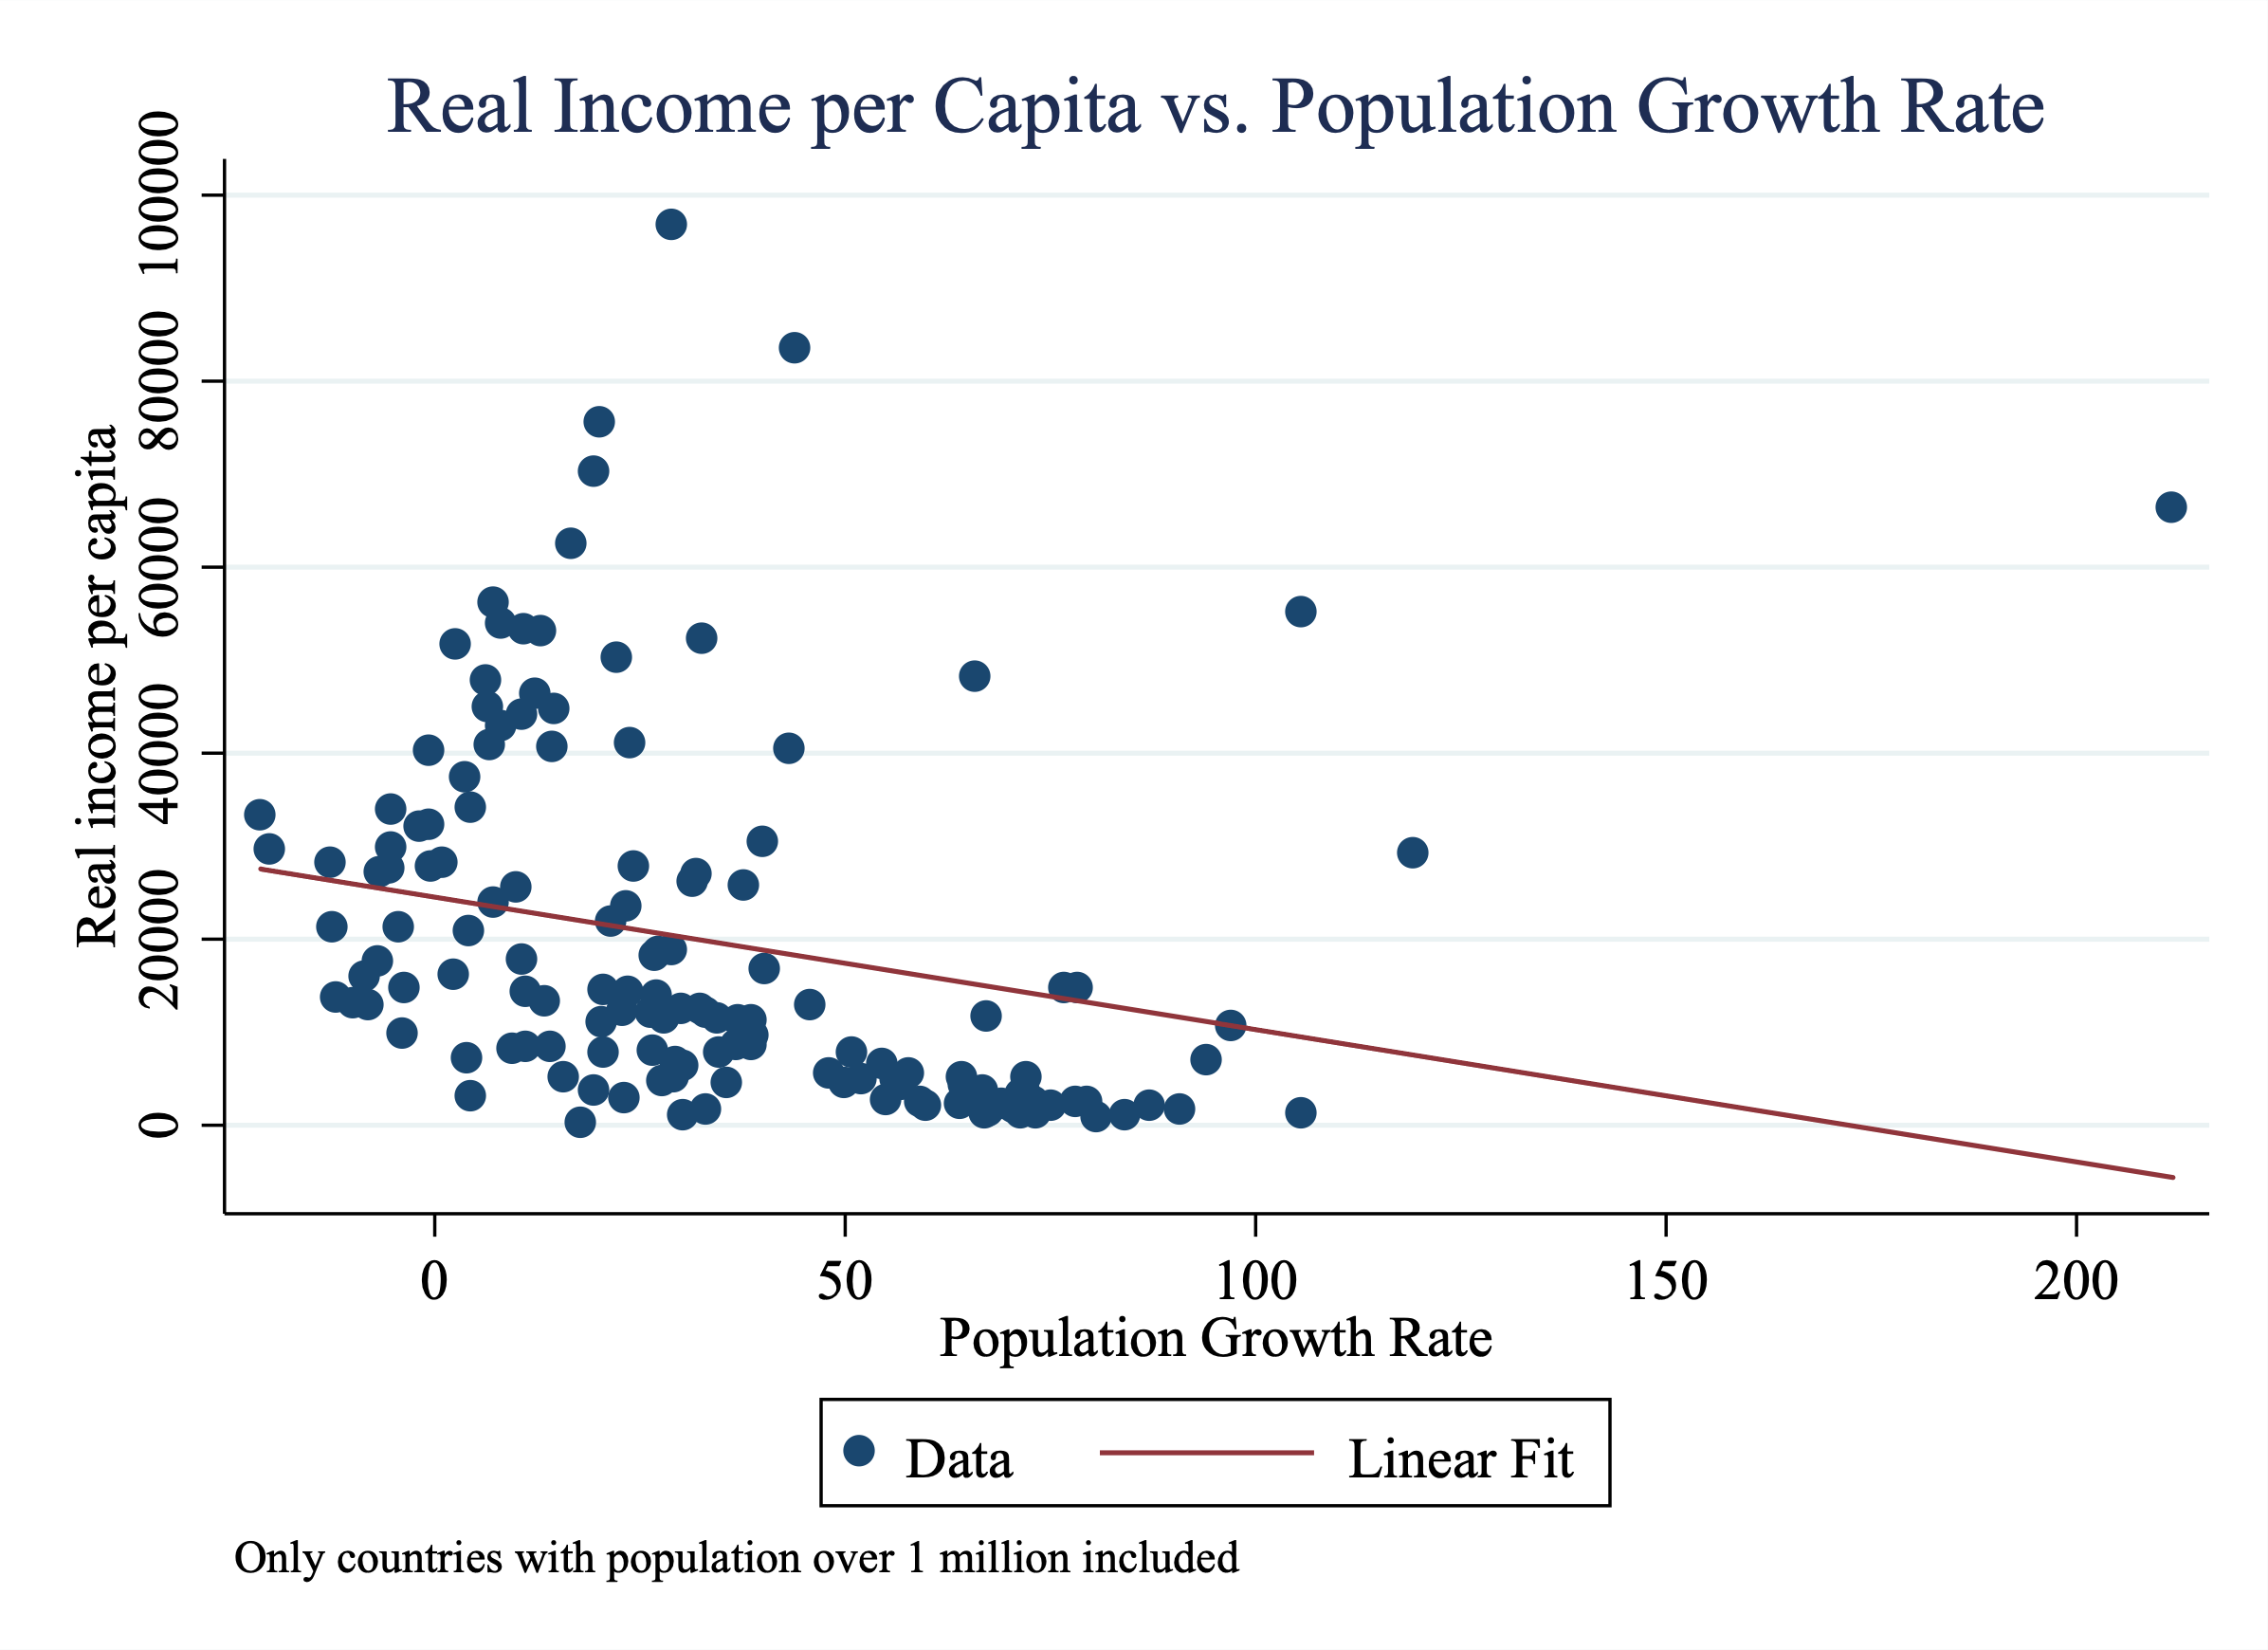
\includegraphics[scale=0.25]{Figures/Fig_7pt2.png}
\end{figure}

\end{frame}

\begin{frame}
\frametitle[alignment=center]{Growth is uncorrelated with initial level of GDP}
\begin{figure}
\centering
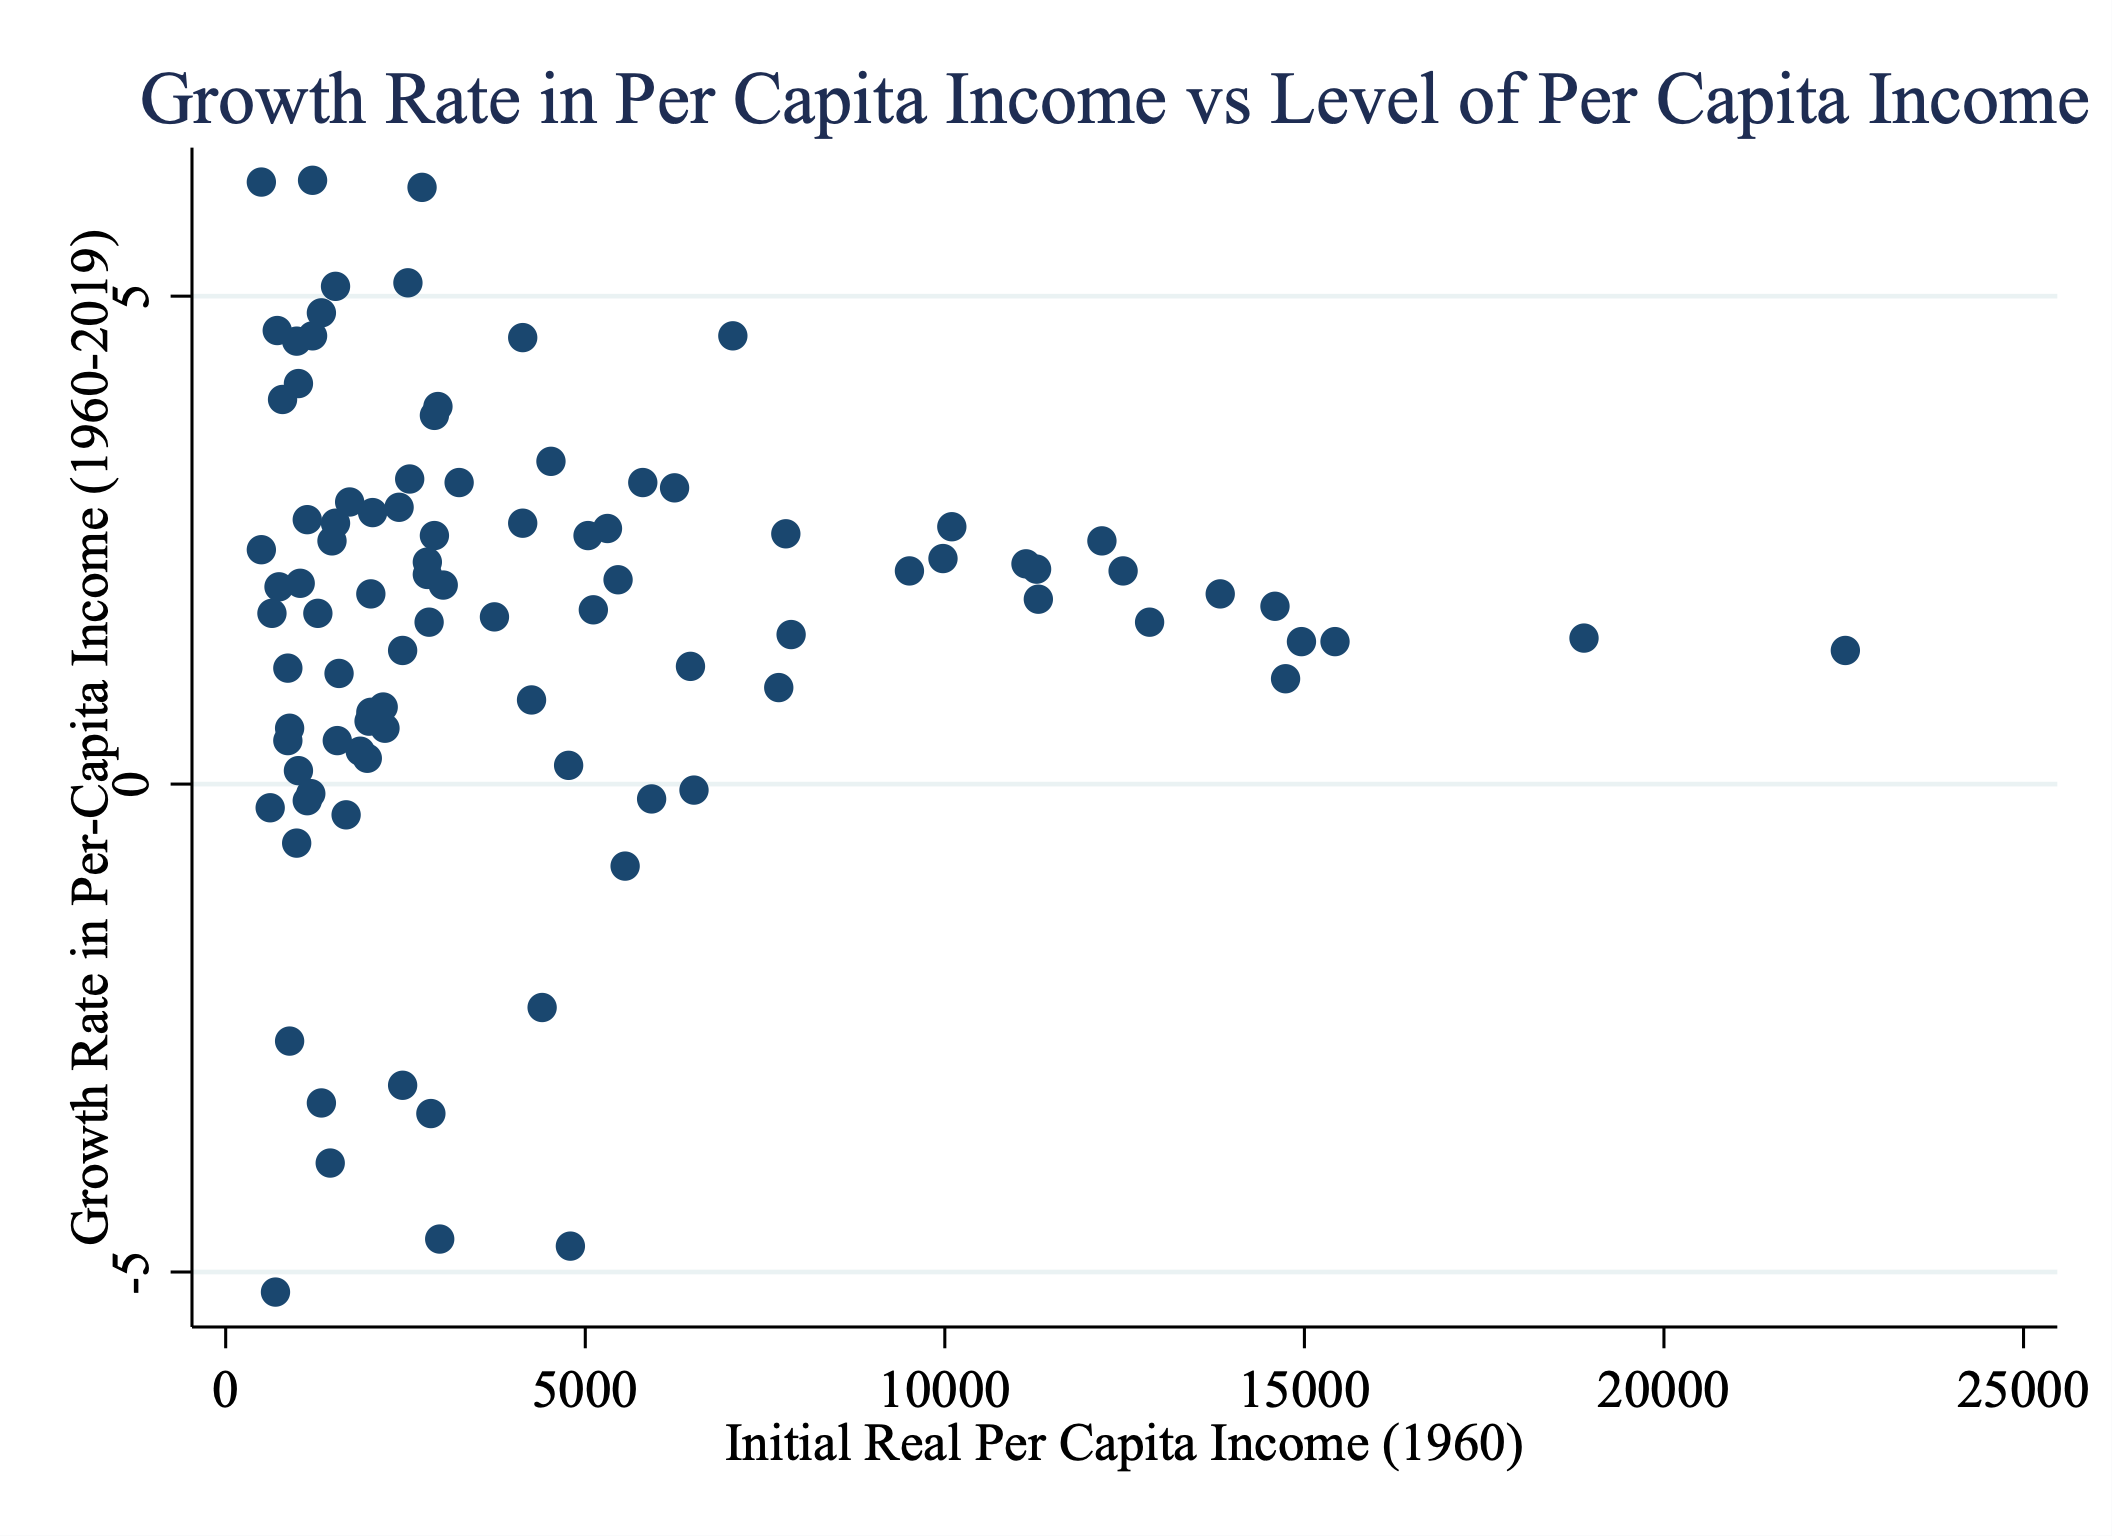
\includegraphics[scale=0.25]{Figures/Fig_7pt3.png}
\end{figure}
 (And is more homogenous among rich countries)
\end{frame}

\begin{frame}
\frametitle[alignment=center]{Growth is uncorrelated with initial level of GDP}
\begin{figure}
\centering
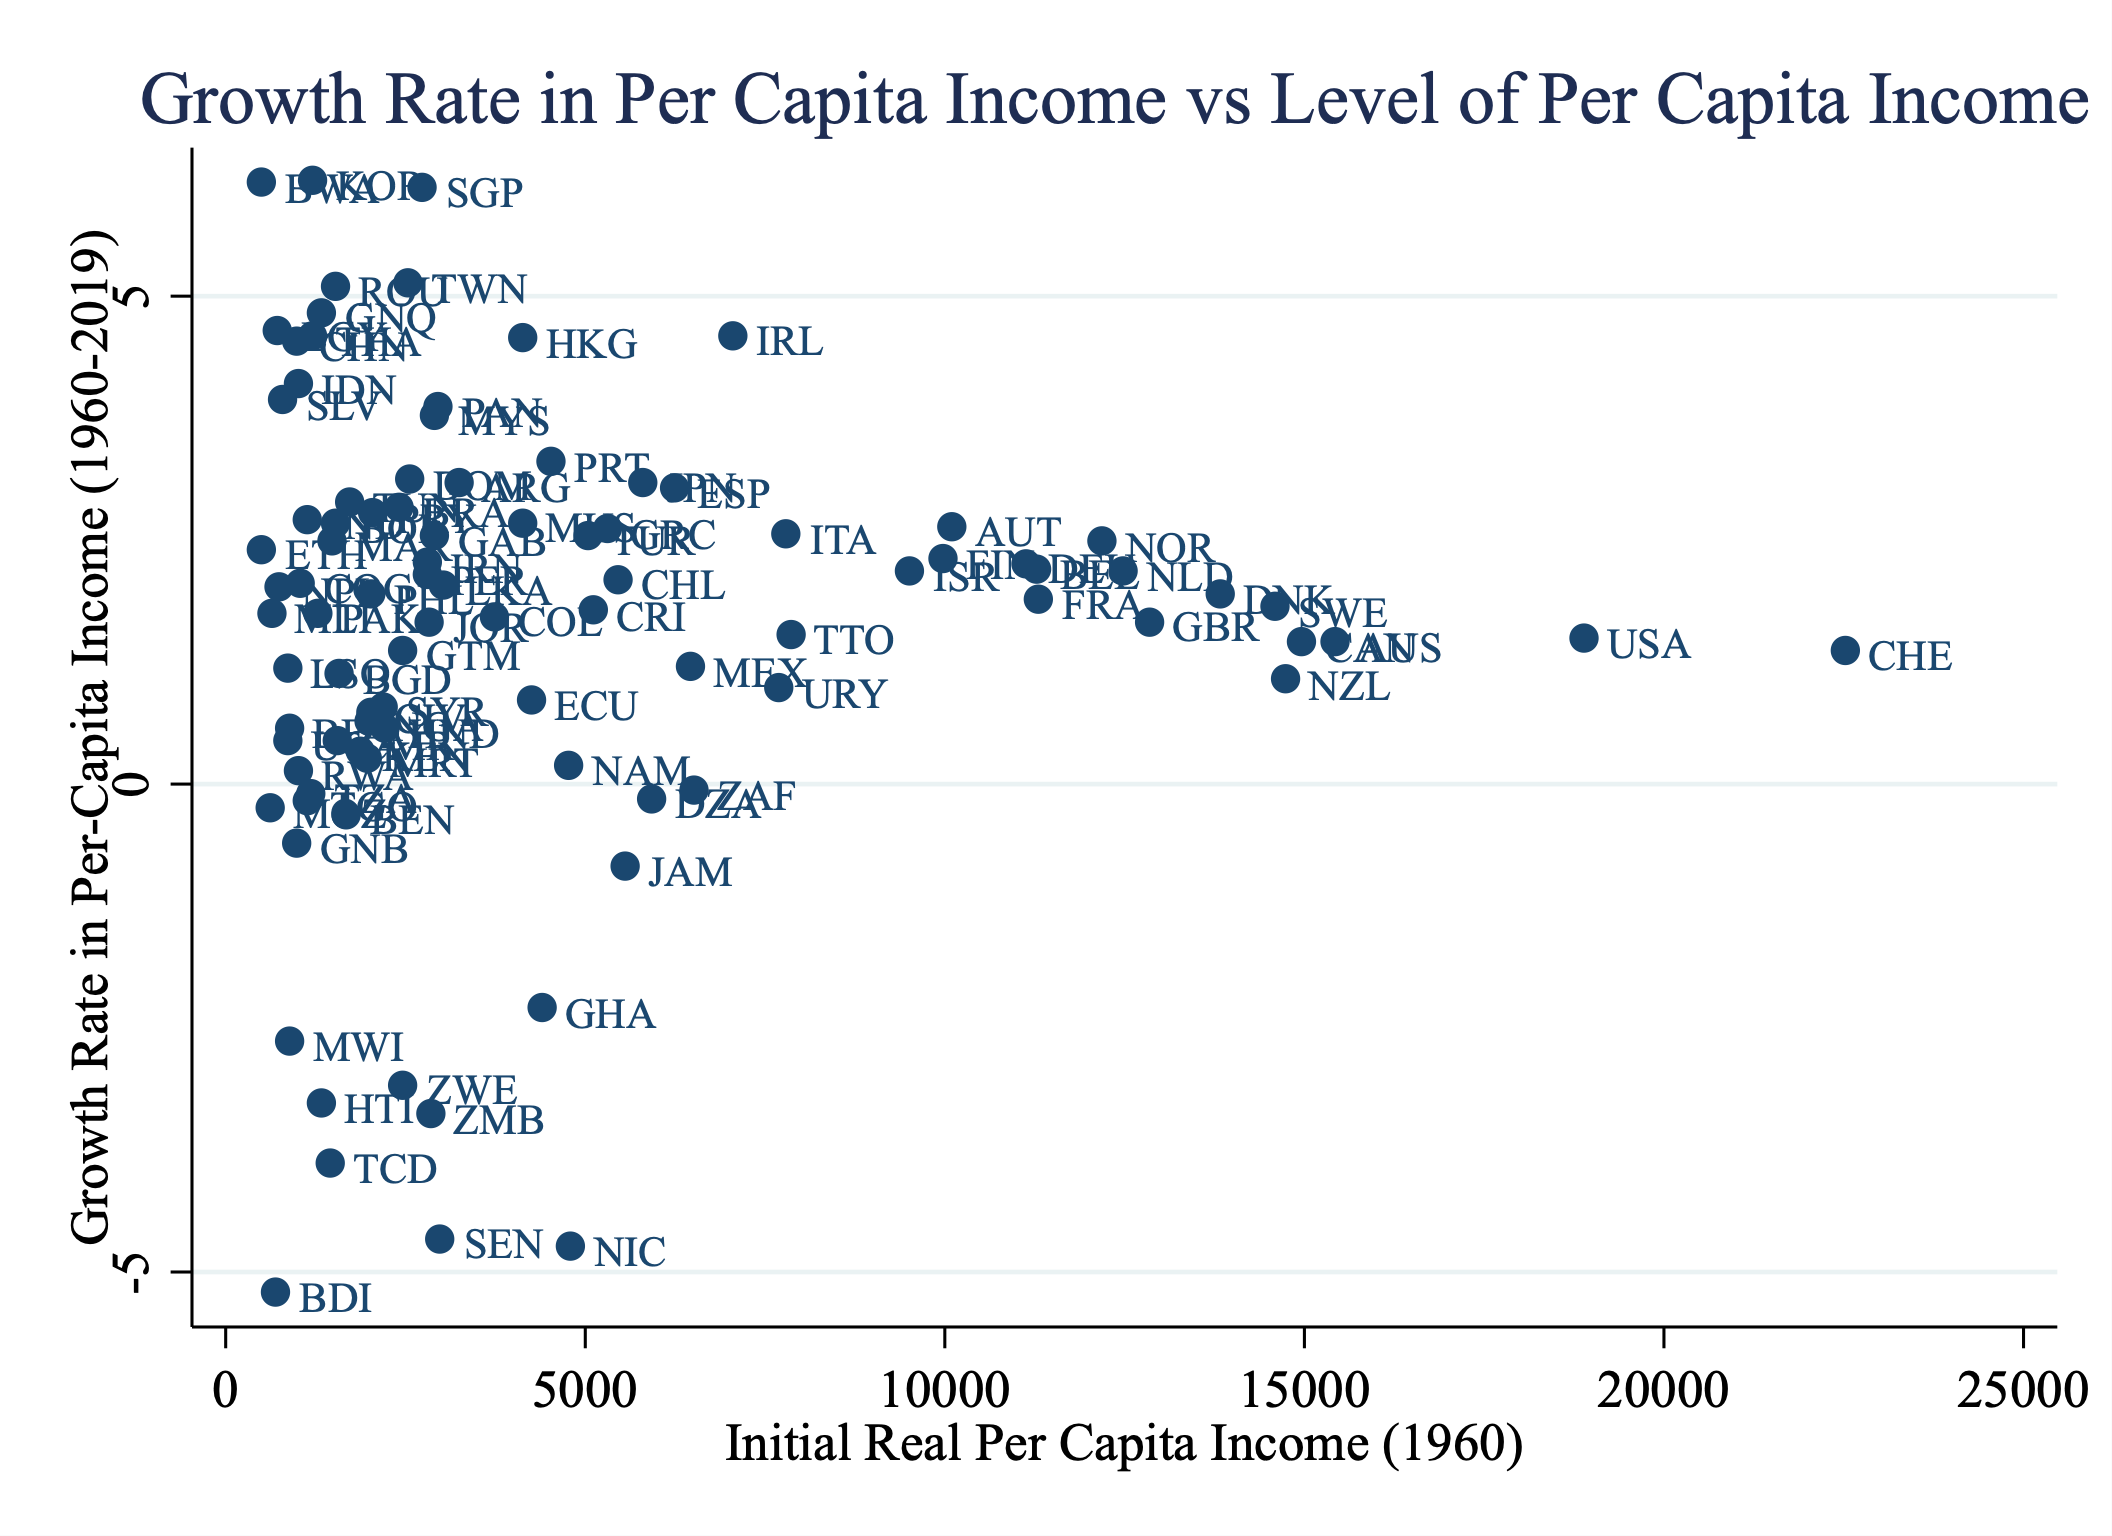
\includegraphics[scale=0.25]{Figures/Fig_7pt3a.png}
\end{figure}
\end{frame}

\begin{frame}
\frametitle[alignment=center]{Malthusian Model of Economic Growth-I}
\begin{itemize}
\item This will be our first model, and it will be terrible
\bigskip
\item Production function $Y$ in terms of TFP $z$, capital (land!) $L$, and labor $N$:
$$Y=zF(L,N)$$
\item Population growth (prime denotes next period):
$$N'=N+\text{Births}-\text{Deaths}$$
\item Or:
$$N'=N+N(\text{birth rate}-\text{death rate})$$
\item But the birth rate, we'll assume, is increasing in consumption per capita $C/N$ (more food, more babies!)
$$\frac{N'}{N}=g\left(\frac{C}{N}\right)$$
\item So need to think about $C/N$
\end{itemize}
\end{frame}

\begin{frame}
\frametitle[alignment=center]{Malthusian Model of Economic Growth-II}
$$\frac{N'}{N}=g\left(\frac{zF(L,N)}{N}\right)$$
\begin{itemize}
\item Or:
$$\frac{N'}{N}=g\left(zF(\frac{L}{N},1)\right)$$
\item But noting that $c=zF(\frac{L}{N},1)$ is per-capita consumption:
$$\frac{N'}{N}=g\left(c)\right)$$
\item Population growth is a function of consumption per capita alone
\end{itemize}
\end{frame}


\begin{frame}
\frametitle[alignment=center]{Population Growth in the Steady State}
\begin{figure}
\centering
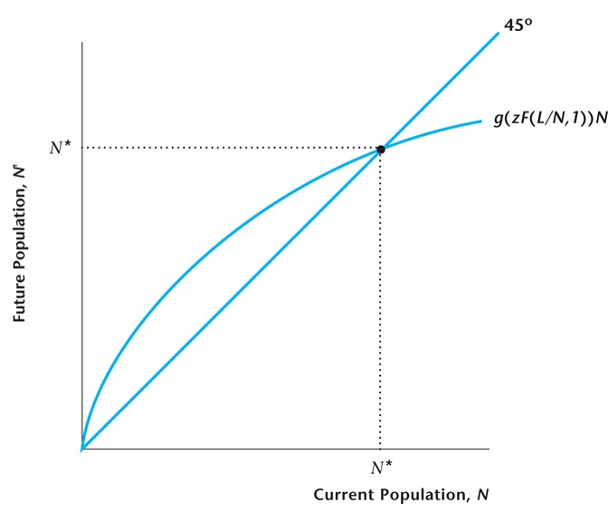
\includegraphics[scale=0.5]{Figures/W_Fig_7pt6.png}
\end{figure}
Consumption has a fixed point!
\end{frame}

\begin{frame}
\frametitle[alignment=center]{Per-Worker Production Function}
\begin{figure}
\centering
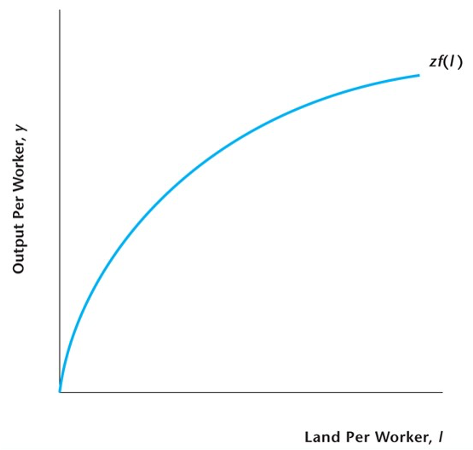
\includegraphics[scale=0.5]{Figures/W_Fig_7pt7.png}
\end{figure}
$$\frac{F(L,N)}{N}=F\left(\frac{L}{N},1\right)=f(l)$$
\end{frame}

\begin{frame}
\frametitle[alignment=center]{Malthusian Model Steady State}
\begin{figure}
\centering
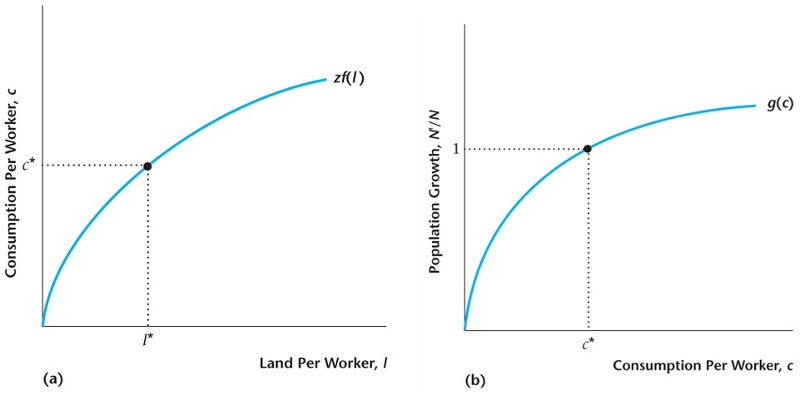
\includegraphics[scale=0.5]{Figures/W_Fig_7pt8.png}
\end{figure}
Now we can analyze shocks to the model: $z$ and population control
\end{frame}



\begin{frame}
\frametitle[alignment=center]{Increase in $z$}
\begin{figure}
\centering
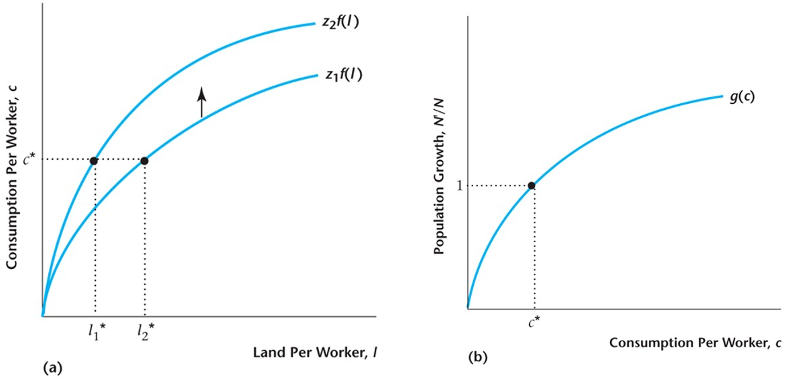
\includegraphics[scale=0.5]{Figures/W_Fig_7pt9.png}
\end{figure}
\end{frame}



\begin{frame}
\frametitle[alignment=center]{Increase in $z$}
\begin{figure}
\centering
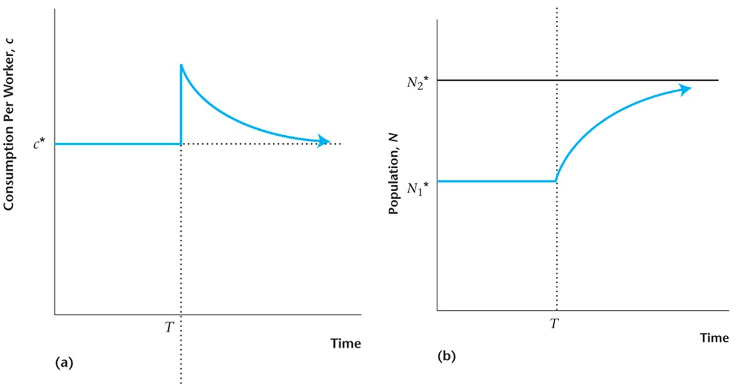
\includegraphics[scale=0.5]{Figures/W_Fig_7pt10.png}
\end{figure}
\end{frame}

\begin{frame}
\frametitle[alignment=center]{Population Control}
\begin{figure}
\centering
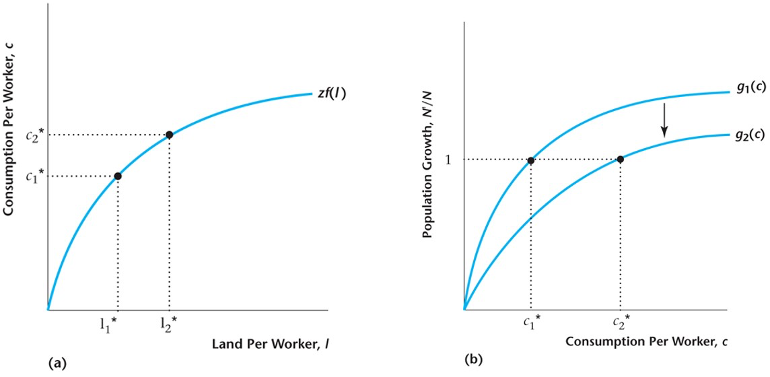
\includegraphics[scale=0.5]{Figures/W_Fig_7pt11.png}
\end{figure}
\end{frame}


\begin{frame}
\frametitle[alignment=center]{Is the Malthusian model any good?}
\begin{itemize}
\item No!  It's truly terrible
\bigskip
\item But it's a start on modellng growth
\bigskip
\item Main change:  land may be fixed, but capital isn't!  
\bigskip
\item Also, income and population growth are negatively correlated (at the country and the individual level)
\bigskip
\item Issues with assumptions, but method/idea seems sound
\end{itemize}
\end{frame}

\begin{frame}
\frametitle[alignment=center]{Population Growth by Country}
\begin{figure}
\centering
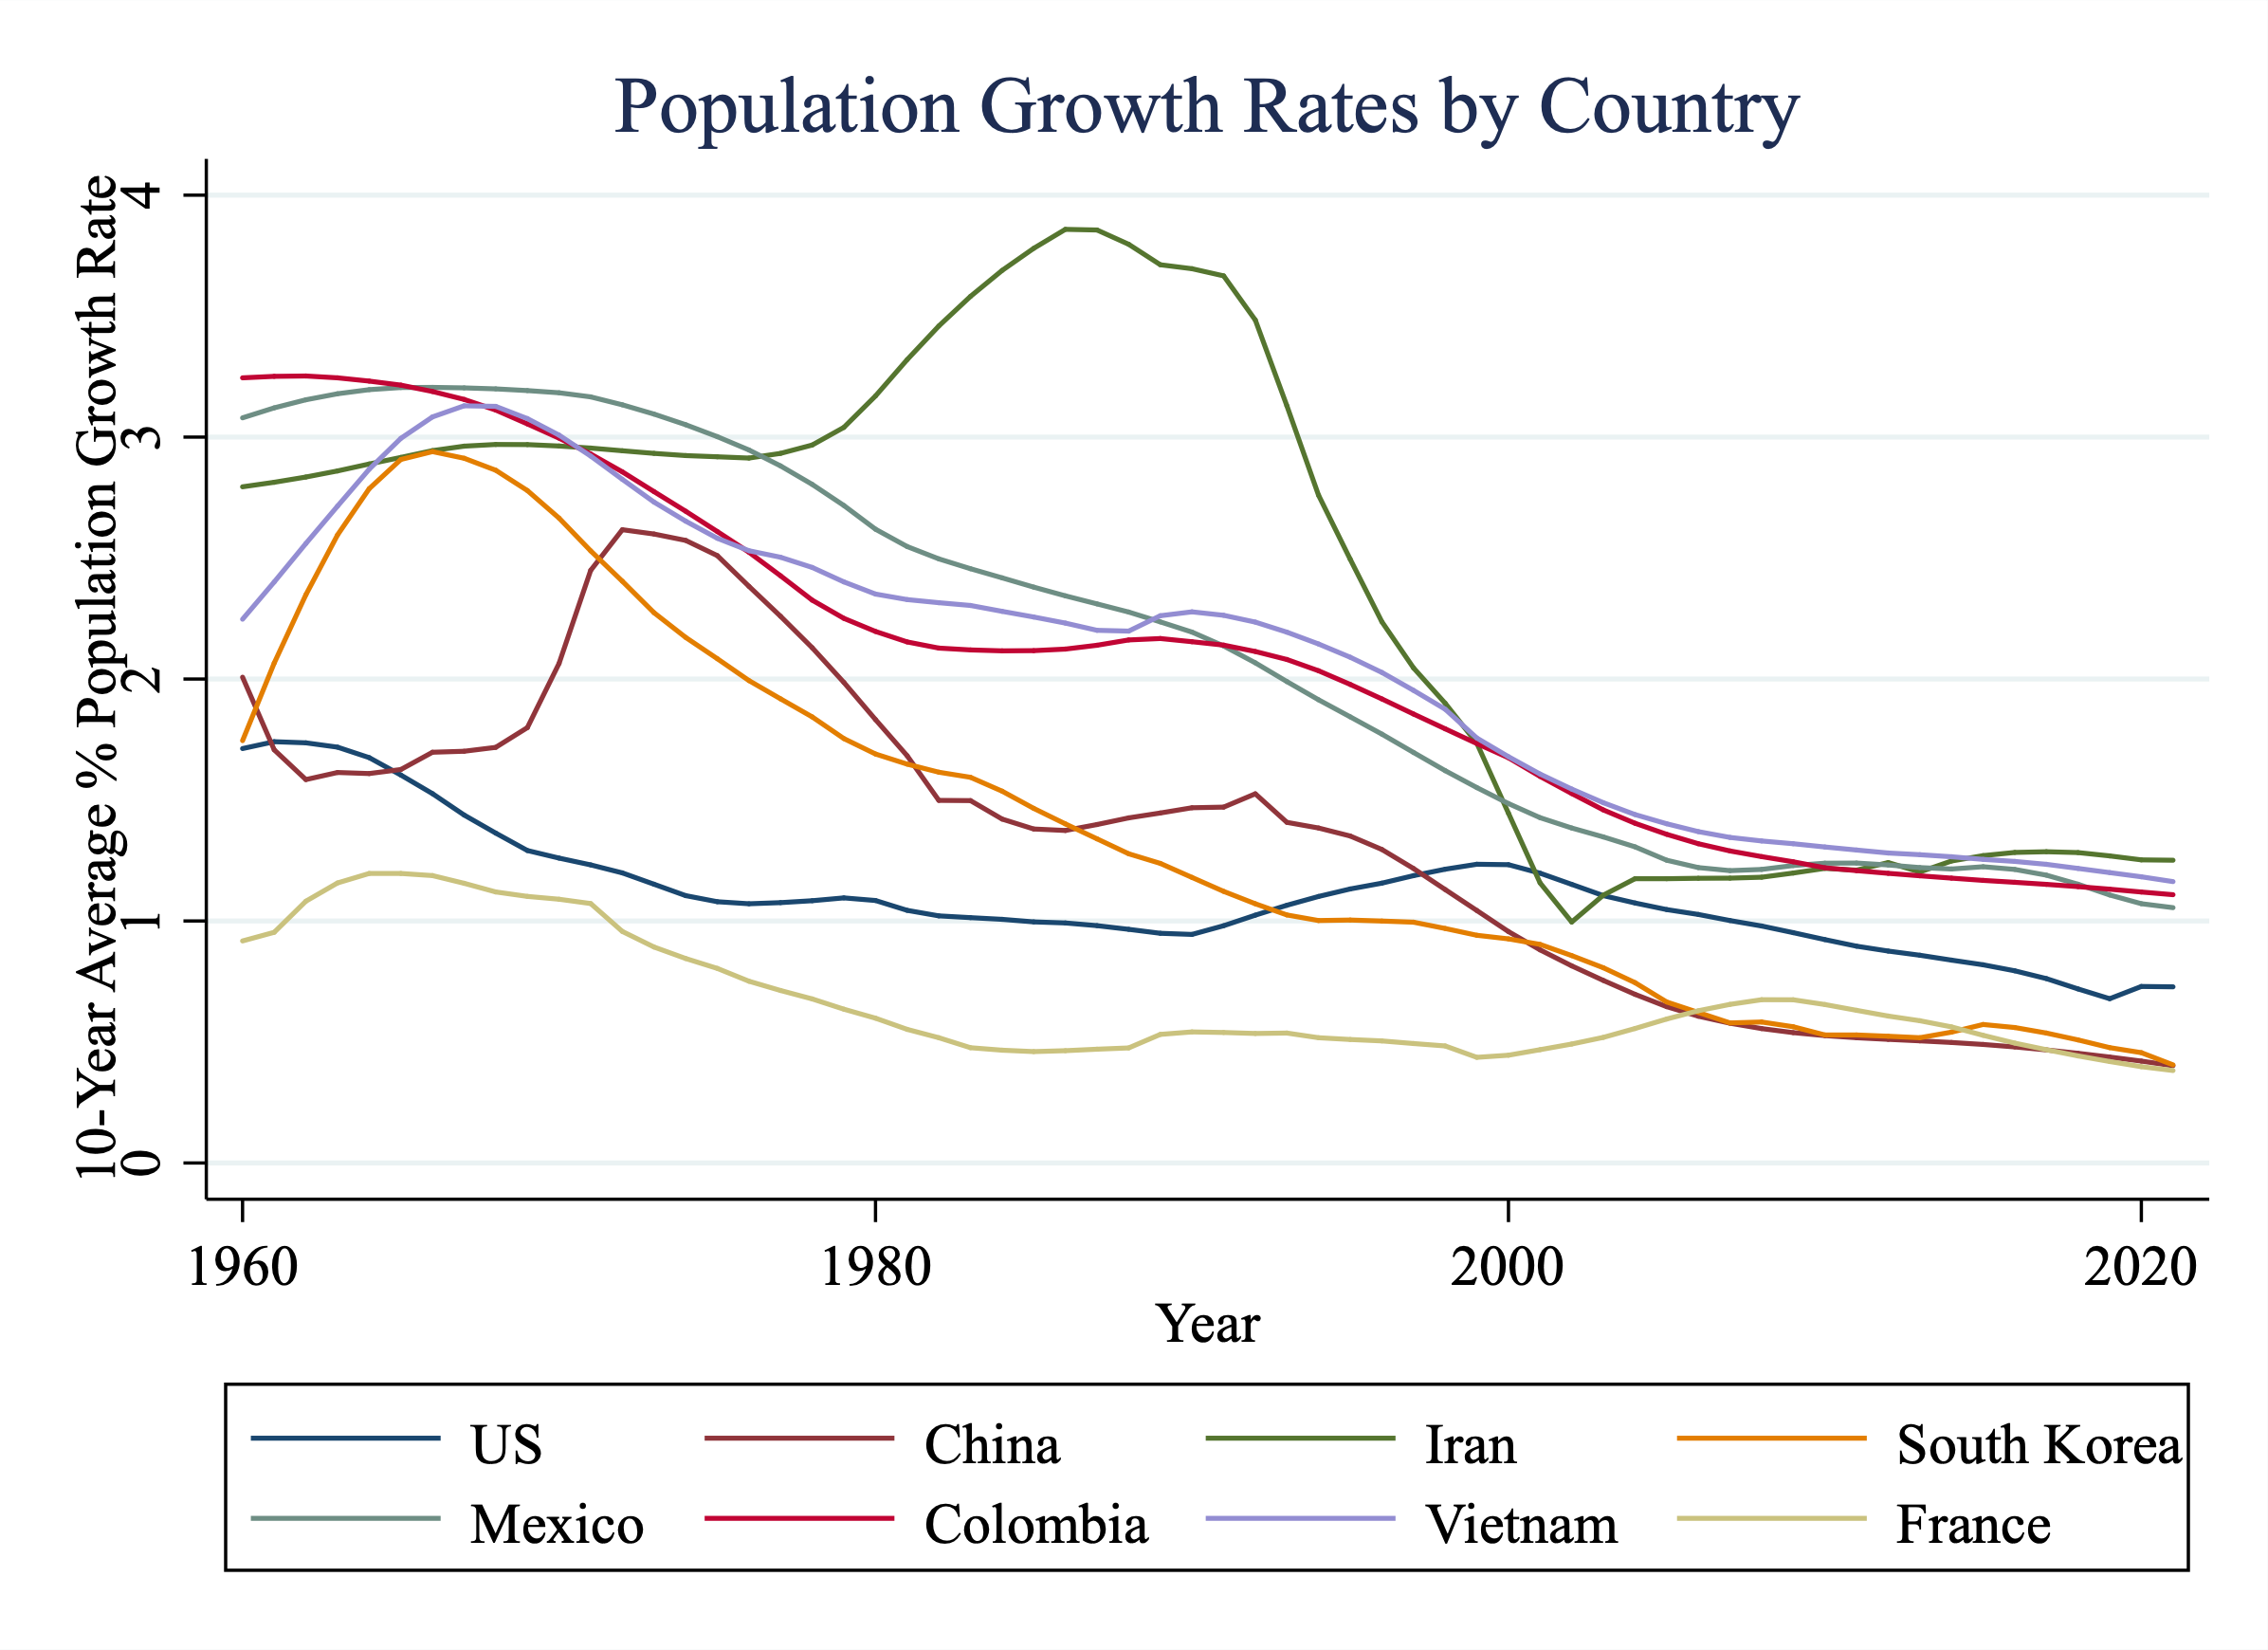
\includegraphics[scale=0.25]{Figures/PopGrowth_country.png}
\end{figure}
\end{frame}


\begin{frame}
\frametitle[alignment=center]{Population Growth by Region}
\begin{figure}
\centering
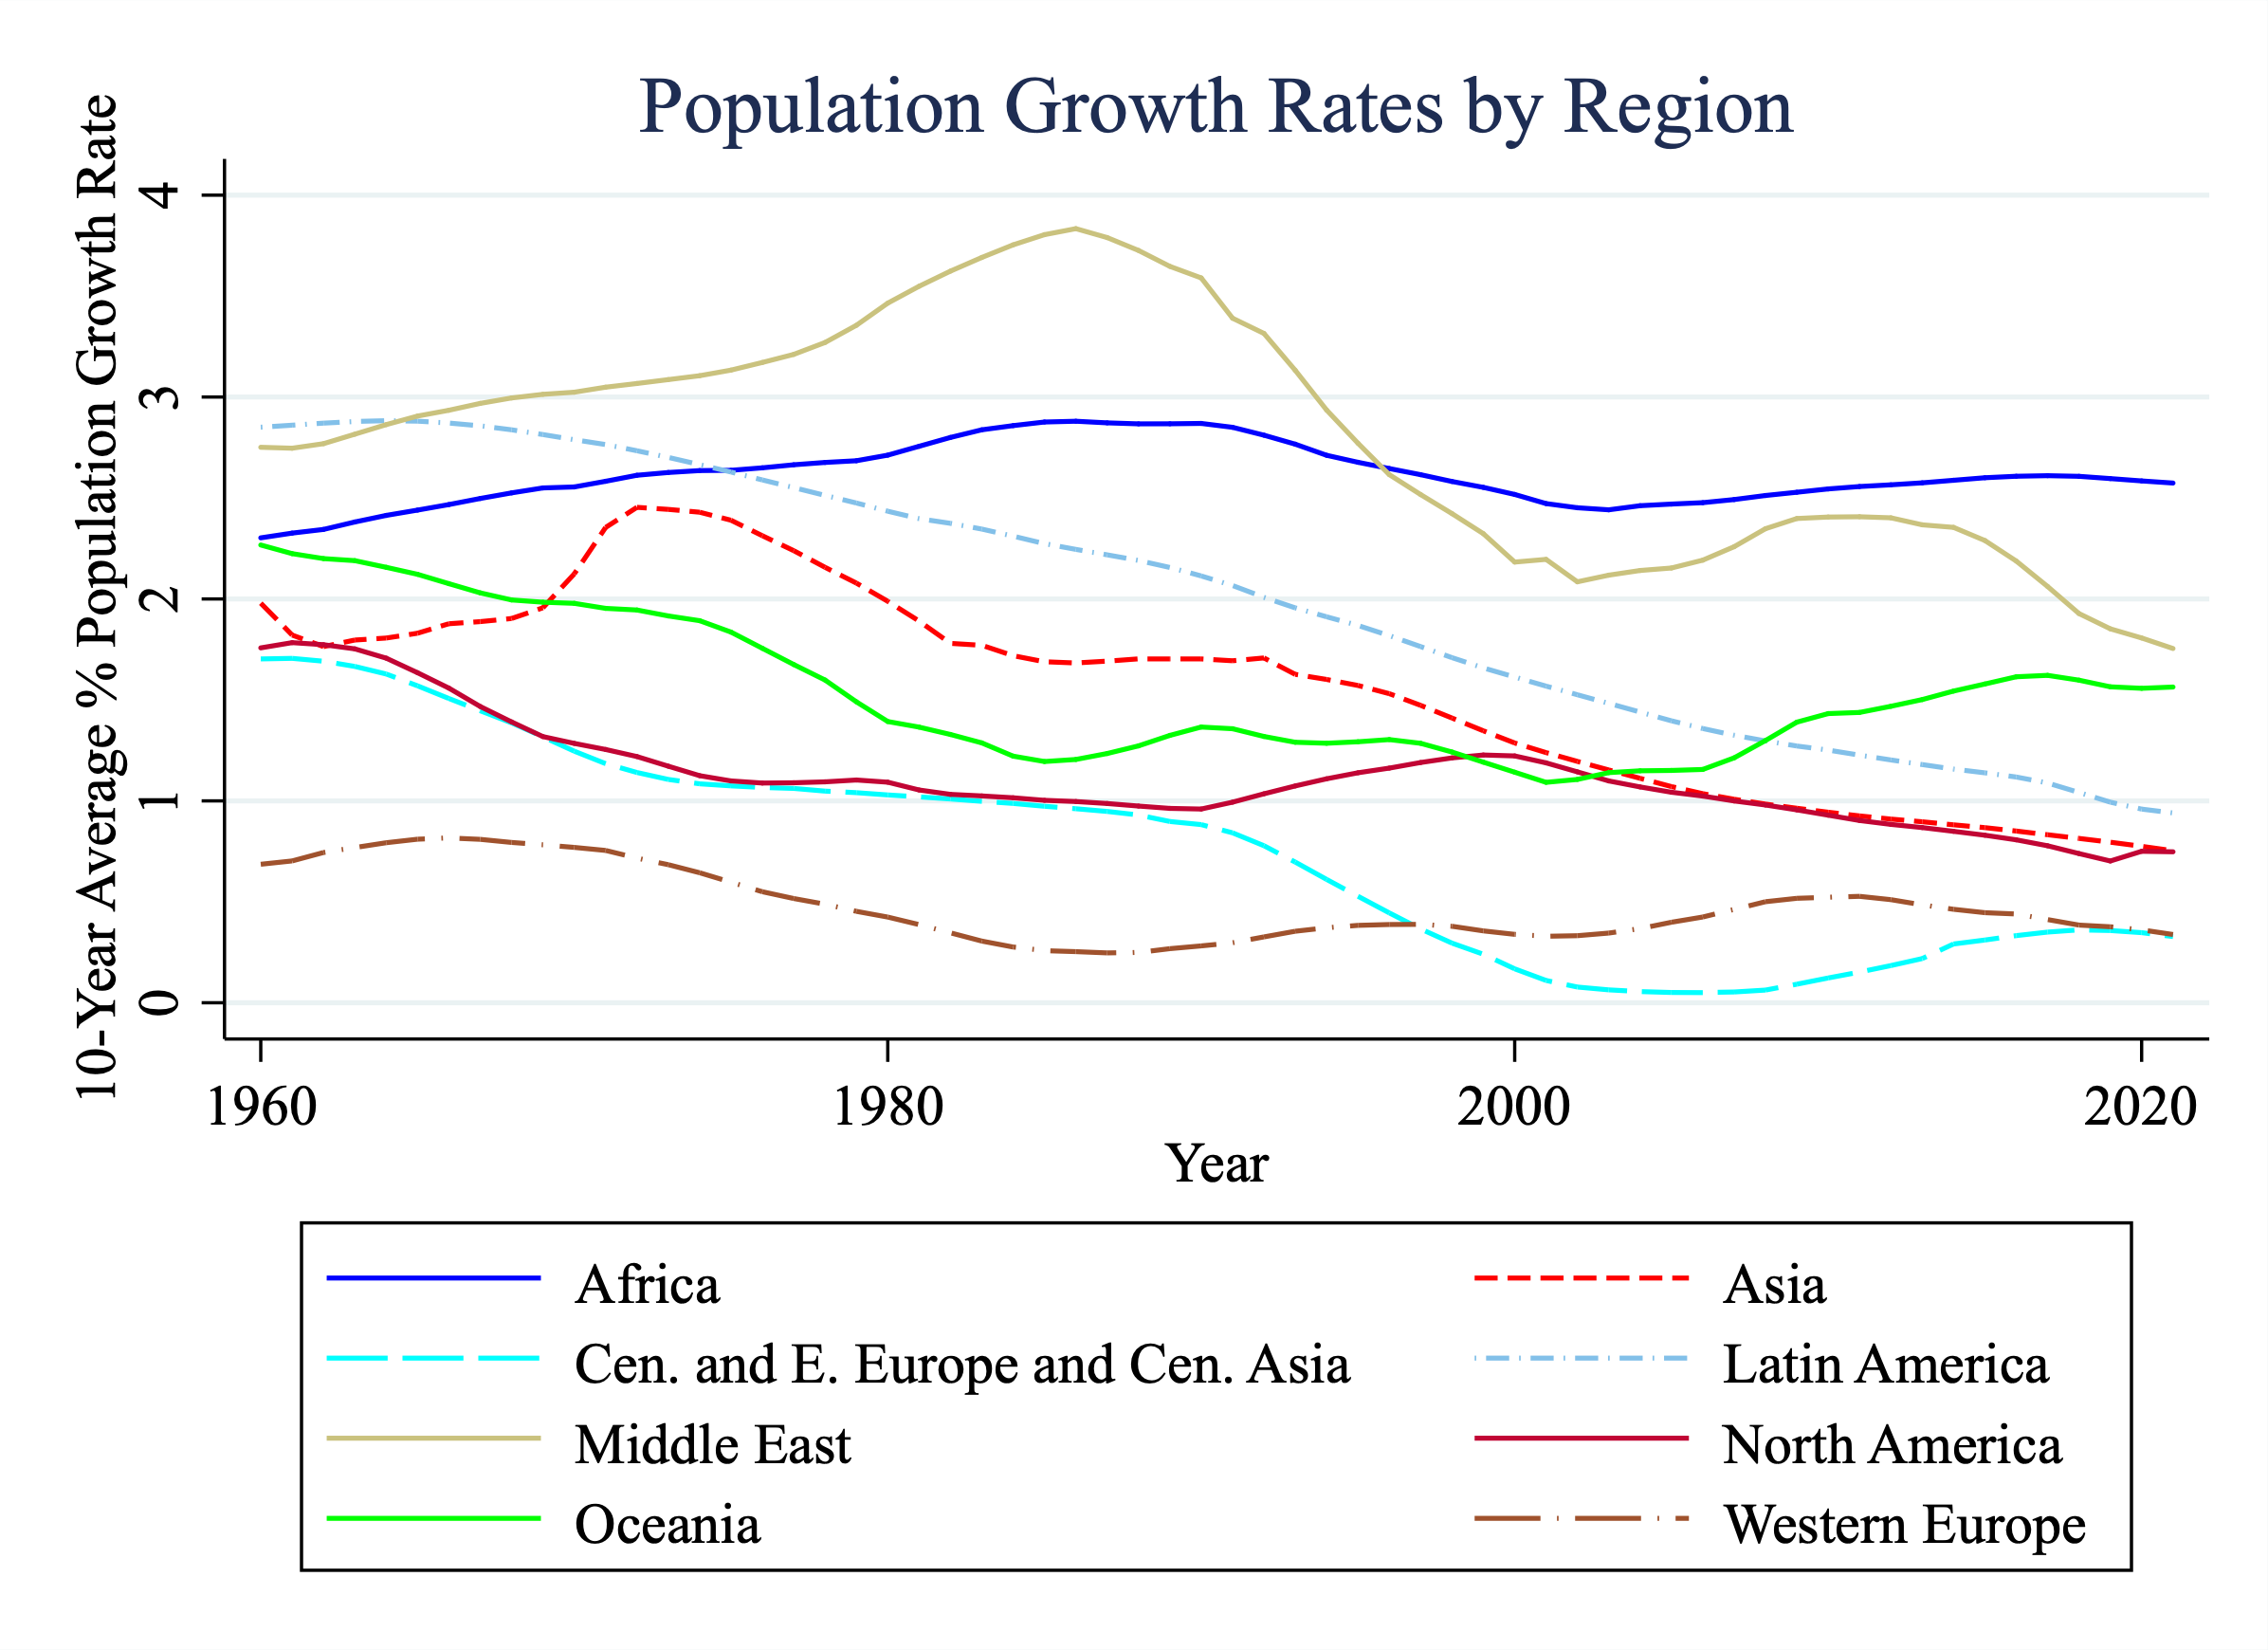
\includegraphics[scale=0.25]{Figures/PopGrowth_region.png}
\end{figure}
\end{frame}

\begin{frame}
\frametitle[alignment=center]{Solow Growth Model-Overview}
\begin{itemize}
\item $z$ is exogenously increasing (changing)
\bigskip
\item Population growth is fixed
\bigskip
\item Savings/consumption are just constant fractions of production  
\bigskip
\item Let it rip
\end{itemize}
\end{frame}


\begin{frame}
\frametitle[alignment=center]{Solow Growth Model-I}
\begin{itemize}
\item Population growth:
$$N'=(1+n)N$$
\item $s$ is fraction of product saved, $1-s$ is fraction consumed
$$C=(1-s)Y$$
\bigskip
\item Firms face the production function:
$$Y=zF(K,N)$$
\item Or in per-capita terms, because CRS:
$$y=zf(k)$$
\item Capital has a law of motion:
$$K'=(1-\delta)K+I$$\end{itemize}
\end{frame}

\begin{frame}
\frametitle[alignment=center]{Solow Growth Model-II}
\begin{itemize}
\item What is equilibrium of model?  
$$Y=C+I$$
\item So, using savings and law of motion of capital:
$$K'=sY+(1-\delta)K$$
\item Substituting in the production function and dividing by $N$:
$$\frac{K'}{N}=sz\frac{F(K,N)}{N}+(1-\delta)\frac{K}{N}$$
\item Multiplying and dividing by $N'$, we get in per-capita terms:
$$k'(1+n)=szf(k)+(1-\delta)k$$
\item Or:
$$k'=\frac{szf(k)}{1+n}+\frac{(1-\delta)k}{1+n}$$
\item Now we have how capital moves as a function of capital, can graph for equilibrium
\end{itemize}
\end{frame}


\begin{frame}
\frametitle[alignment=center]{Determination of the Steady State Quantity of Capital Per Worker}
\begin{figure}
\centering
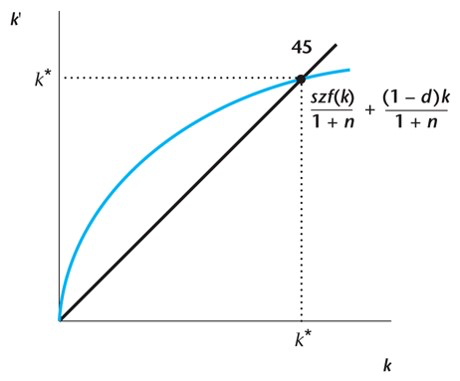
\includegraphics[scale=0.5]{Figures/W_Fig_7pt13.png}
\end{figure}
\end{frame}

\begin{frame}
\frametitle[alignment=center]{Analyzing the Steady State}
\begin{itemize}
\item In the steady state, $k^*=k'=k$, so:
$$k^*=\frac{szf(^*)}{1+n}+\frac{(1-\delta)^*}{1+n}$$
\item Or:
$$szf(k^*)=(n+\delta)k^*$$
\end{itemize}
\end{frame}



\begin{frame}
\frametitle[alignment=center]{Determination of the Steady State Quantity of Capital Per Worker}
\begin{figure}
\centering
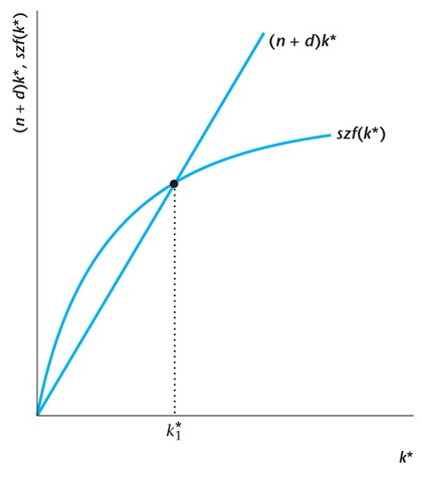
\includegraphics[scale=0.5]{Figures/W_Fig_7pt14.png}
\end{figure}
\end{frame}
'
\begin{frame}
\frametitle[alignment=center]{Effect of an Increase in Savings on the Steady State Quantity of Capital per Worker}
\begin{figure}
\centering
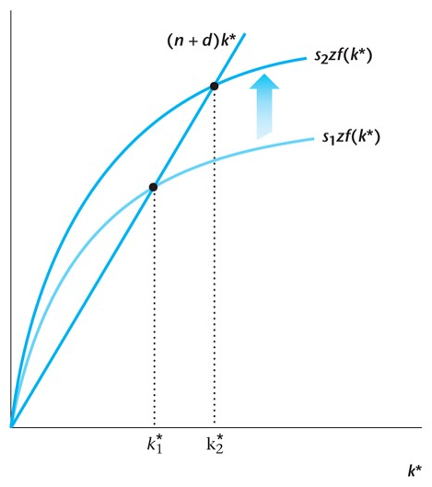
\includegraphics[scale=0.5]{Figures/W_Fig_7pt15.png}
\end{figure}
\end{frame}

'
\begin{frame}
\frametitle[alignment=center]{Effect of an Increase in the Savings Rate at time T}
\begin{figure}
\centering
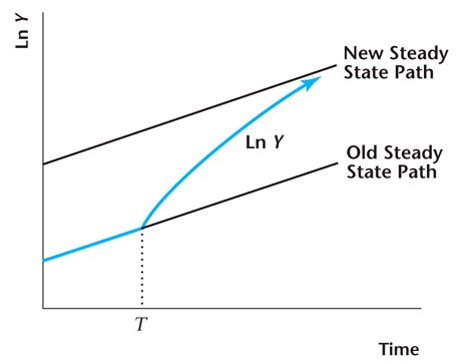
\includegraphics[scale=0.5]{Figures/W_Fig_7pt16.png}
\end{figure}
\end{frame}

\begin{frame}
\frametitle[alignment=center]{Steady State consumption per worker}
\begin{figure}
\centering
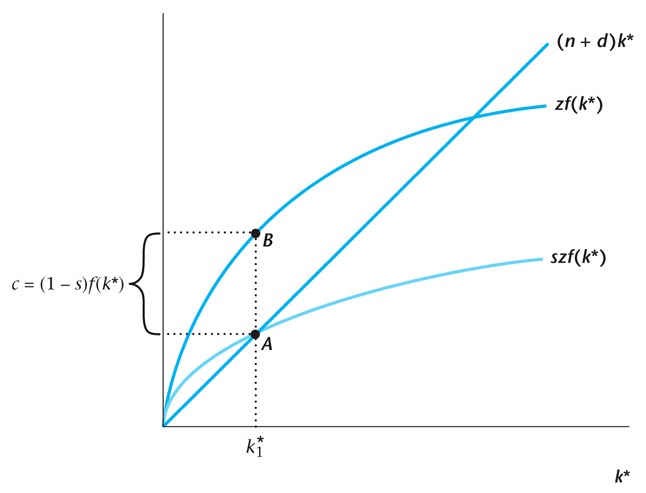
\includegraphics[scale=0.5]{Figures/W_Fig_7pt17.png}
\end{figure}
\end{frame}


\begin{frame}
\frametitle[alignment=center]{Golden Rule Quantity of Capital per Worker}
\begin{figure}
\centering
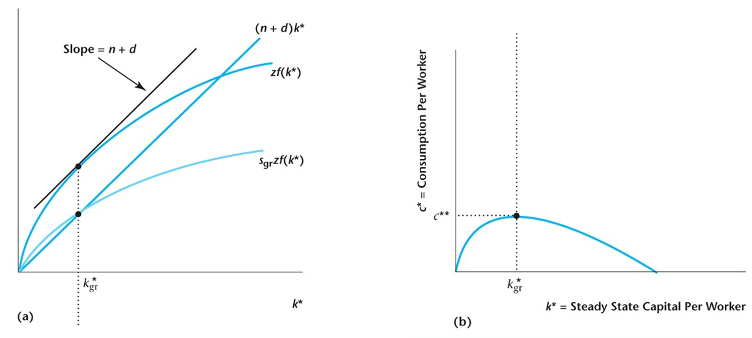
\includegraphics[scale=0.5]{Figures/W_Fig_7pt18.png}
\end{figure}
\end{frame}

\begin{frame}
\frametitle[alignment=center]{Steady State Effects of an Increase in Labor Force Growth Rate}
\begin{figure}
\centering
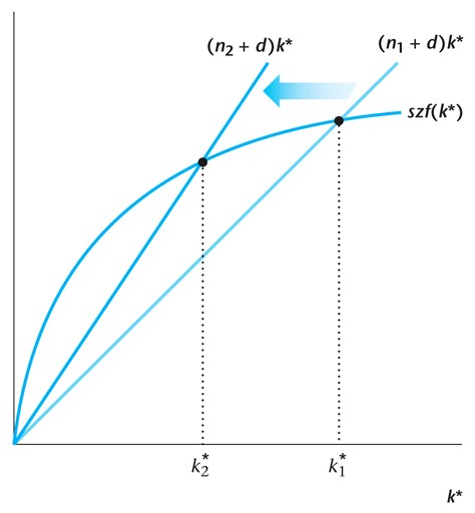
\includegraphics[scale=0.5]{Figures/W_Fig_7pt19.png}
\end{figure}
\end{frame}

\begin{frame}
\frametitle[alignment=center]{Steady State Effects of an Increase in Productivity}
\begin{figure}
\centering
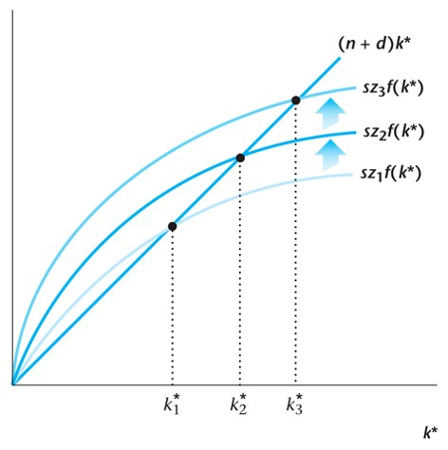
\includegraphics[scale=0.5]{Figures/W_Fig_7pt20.png}
\end{figure}
\end{frame}


\begin{frame}
\frametitle[alignment=center]{Breaking from Trend}
\begin{figure}
\centering
\includegraphics[scale=0.5]{Figures/W_Fig_7pt21.png}
\end{figure}
\end{frame}

\begin{frame}
\frametitle[alignment=center]{Breaking from Trend}
\begin{figure}
\centering
\includegraphics[scale=0.5]{Figures/W_Fig_7pt22.png}
\end{figure}
\end{frame}

\begin{frame}
\frametitle[alignment=center]{Breaking from Trend}
\begin{figure}
\centering
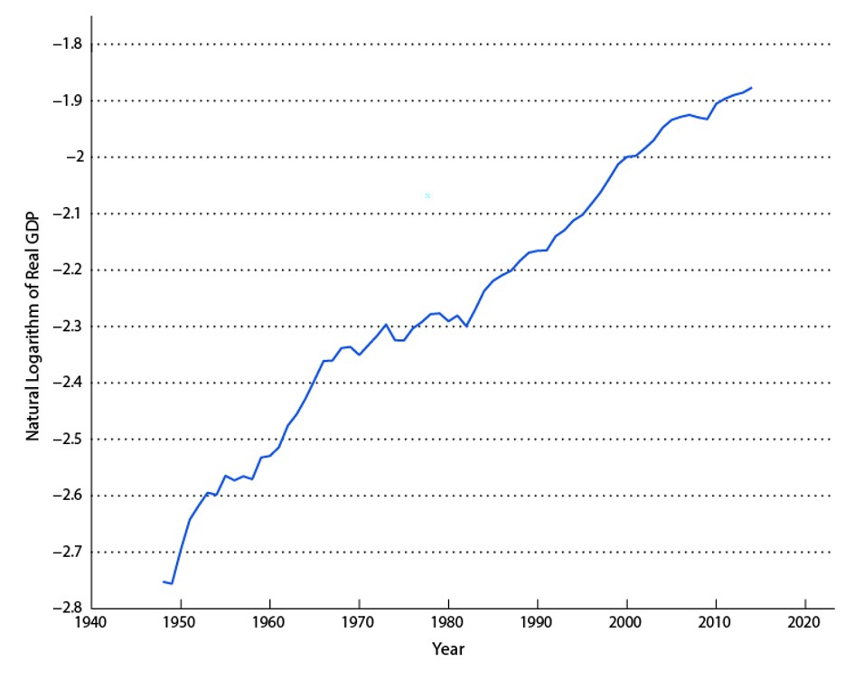
\includegraphics[scale=0.5]{Figures/W_Fig_7pt23.png}
\end{figure}
\end{frame}

\begin{frame}
\frametitle[alignment=center]{Growth Accounting}
\begin{itemize}
\item Read Williamson 7.7 and complete the updated exercise in the homework.
\end{itemize}
\end{frame}





\end{document}